% Scope-controlled review, 27 November 2026.
% Source snapshot: codex/final 391c5f4d0e5ea3a5341aab414ac1944e8e46f0c4 and the newer local author compact manuscript.
% Preserve WKU 12pt single spacing and the author declaration unsigned.
% Editorial additions and replacements marked with \review; red denotes key equations.
% The pinned source snapshot and conditional results are distinguished from fresh training.
\documentclass[12pt,a4paper,oneside]{report}
\usepackage[T1]{fontenc}
\usepackage[utf8]{inputenc}
\usepackage[english]{babel}
\usepackage{lmodern}
\usepackage[nopatch=footnote]{microtype}
\usepackage[top=1in,bottom=0.689in,hmargin=1.25in,nohead,includefoot,foot=0.311in,footskip=0.5827in]{geometry}
\usepackage{amsmath,amssymb,amsthm,mathtools,mathrsfs}
\usepackage{booktabs,array,tabularx,longtable}
\renewcommand{\tabularxcolumn}[1]{>{\raggedright\arraybackslash}p{#1}}
\usepackage{graphicx,tikz,pgfplots,pgfplotstable,adjustbox}
\BeforeBeginEnvironment{tikzpicture}{\begin{adjustbox}{max width=\linewidth}}
\AfterEndEnvironment{tikzpicture}{\end{adjustbox}}
\usetikzlibrary{arrows.meta,positioning,calc}
\usepgfplotslibrary{groupplots,fillbetween}
\pgfplotsset{compat=1.18}
\usepackage[numbers,sort&compress]{natbib}
\usepackage[hyphens]{url}
\usepackage{hyperref,bookmark}
\usepackage{fancyhdr,titlesec,caption,placeins}
\definecolor{ink}{HTML}{263B5E}
\definecolor{teal}{HTML}{087F8C}
\definecolor{warm}{HTML}{B65528}
\definecolor{keyred}{HTML}{AB2634}
\definecolor{authorblue}{HTML}{1748A4}
\newcommand{\authornote}[1]{\textcolor{authorblue}{\textit{(#1)}}}
\newcommand{\keyeq}[1]{\textcolor{keyred}{#1}}
\hypersetup{colorlinks=true,linkcolor=ink,citecolor=teal,urlcolor=teal,
 pdfauthor={Yihong Xiao},
 pdftitle={Parameter-Dependent Lie Symmetries and Semi-Analytical Solutions of Nonlinear PDEs},
 pdfsubject={Undergraduate dissertation, MATH 4890}}
\titleformat{\chapter}[hang]{\normalfont\Large\bfseries\raggedright}{\thechapter.}{.7em}{}
\titlespacing*{\chapter}{0pt}{-20pt}{12pt}
\titleformat{\section}{\normalfont\large\bfseries}{\thesection.}{.6em}{}
\titleformat{\subsection}{\normalfont\normalsize\bfseries}{\thesubsection.}{.6em}{}
\titlespacing*{\section}{0pt}{10pt plus 2pt}{4pt}
\titlespacing*{\subsection}{0pt}{9pt plus 2pt}{3pt}
\captionsetup{font=small,labelfont=bf,skip=4pt}
\setlength{\textfloatsep}{11pt plus 2pt minus 2pt}
\setlength{\intextsep}{10pt plus 2pt minus 2pt}
\renewcommand{\topfraction}{.9}
\renewcommand{\textfraction}{.08}
\setlength{\emergencystretch}{2em}
\setlength{\parskip}{0pt}
\setcounter{tocdepth}{2}
\makeatletter
\renewcommand{\@pnumwidth}{2.8em}
\renewcommand{\@tocrmarg}{3.8em}
\makeatother
\raggedbottom
\numberwithin{equation}{chapter}
\newtheorem{theorem}{Theorem}[chapter]
\newtheorem{proposition}[theorem]{Proposition}
\newtheorem{corollary}[theorem]{Corollary}
\theoremstyle{definition}
\newtheorem{definition}[theorem]{Definition}
\newtheorem{example}[theorem]{Example}
\newtheorem{counterexample}[theorem]{Counterexample}
\theoremstyle{remark}\newtheorem{remark}[theorem]{Remark}
\newcommand{\dd}{\,\mathrm d}
\newcommand{\E}{\mathcal E}
\newcommand{\pr}{\operatorname{pr}}
\newcommand{\rank}{\operatorname{rank}}
\newcommand{\norm}[1]{\left\lVert#1\right\rVert}
\DeclareRobustCommand{\code}[1]{\nolinkurl{#1}}
\newif\ifreviewmarks
\reviewmarkstrue
\DeclareRobustCommand{\review}[1]{{\ifreviewmarks\color{authorblue}\fi #1}}
\DeclareRobustCommand{\revew}[1]{\review{#1}}
\pdfstringdefDisableCommands{\def\review#1{#1}\def\revew#1{#1}}
\newcommand{\doi}[1]{\href{https://doi.org/#1}{doi: #1}}
\pagestyle{fancy}\fancyhf{}
\renewcommand{\headrulewidth}{0pt}
\fancyfoot[R]{\thepage}
\fancypagestyle{plain}{\fancyhf{}\fancyfoot[R]{\thepage}\renewcommand{\headrulewidth}{0pt}}
\setlength{\tabcolsep}{1mm}
\renewcommand{\arraystretch}{1.3}
\addto\captionsenglish{\renewcommand{\bibname}{References}}
\renewcommand{\chaptermark}[1]{\markboth{\thechapter.\ #1}{}}
\tikzset{box/.style={draw=ink,fill=ink!4,rounded corners=2pt,
 align=center,inner sep=5pt,font=\small},
 planned/.style={box,draw=teal,fill=teal!5,dashed},
 arr/.style={-{Latex[length=2mm]},thick,ink},
 warnbox/.style={draw=warm,fill=warm!5,rounded corners=2pt,align=center,inner sep=4pt,font=\scriptsize},
 mlbox/.style={draw=teal,fill=teal!6,rounded corners=2pt,align=center,inner sep=4pt,font=\scriptsize},
 note/.style={font=\scriptsize,align=center},
 warr/.style={-{Latex[length=1.8mm]},thick,warm,dashed},
 tarr/.style={-{Latex[length=1.8mm]},thick,teal}}

\begin{document}
\hypersetup{pageanchor=false}
\pagenumbering{Roman}
\begin{titlepage}
\thispagestyle{plain}
\noindent\IfFileExists{wku_programme_header.pdf}{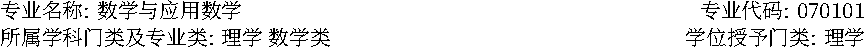
\includegraphics[width=\textwidth]{wku_programme_header.pdf}}{\textbf{Programme in Mathematical Sciences}\par\smallskip\hrule}
\bigskip\bigskip\bigskip\bigskip

\begin{center}
\textbf{College of Science, Mathematics and Technology}\par
\bigskip
\textbf{Wenzhou-Kean University}\par
\bigskip\bigskip
\IfFileExists{WKU.png}{
\includegraphics[width=2.2055in,height=1.9055in]{WKU.png}}{\rule{0pt}{1.9055in}}\par
\bigskip\bigskip\bigskip\bigskip
{\bfseries Parameter-Dependent Lie Symmetries\par
and Semi-Analytical Solutions\par
of Nonlinear PDEs\par}
\bigskip
Saint--Venant--Exner Case Studies\par
Undergraduate Dissertation (MATH 4890)
\end{center}

\bigskip\bigskip
\noindent\begin{minipage}{\textwidth}
\raggedright
\textbf{Student Name:} \underline{Yihong Xiao}\\[8pt]
\textbf{Student ID:} \underline{1308225}\\[8pt]
\textbf{Major:} \underline{Mathematical Sciences (Data Analytics Option)}\\[8pt]
\textbf{Supervisor:} \underline{Dr.\ Puneet Rana}\\[8pt]
\textbf{Date of Submission:} \underline{November 27, 2026}
\end{minipage}
\end{titlepage}
\hypersetup{pageanchor=true}
\setcounter{page}{2}
\chapter*{Author's Declaration}
\addcontentsline{toc}{chapter}{Author's Declaration}

I, the undersigned, hereby declare that this submission is entirely my own work, in my own words, and that all sources used in researching it are fully acknowledged and all quotations properly identified. It has not been submitted, in whole or in part, by me or another person, for the purpose of obtaining any other credit/grade. I have a citation to AI system used to generate the text if I used AI-generated text. I understand the ethical implications of my research, and this work meets the requirements of College of Science, Mathematics and Technology.

\bigskip
\noindent\textbf{AI assistance disclosure.}
\review{ChatGPT assisted with mathematical exposition, the planar potential formulation, the saddle determinant, benchmark design and this editorial revision. Claude Opus 5.5 assisted in developing the SymPy reducer, planar symbolic checks, approximation code and interval checker. Gemini assisted with prose and figures; Grok reviewed scripts. The numerical results reported here come from the project's recorded runs, not from new training in this revision. The scope and data of those runs are documented in Appendix~\ref{app:reproducibility}.}

\authornote{Author: confirm this disclosure, your own derivations and responsibility for the manuscript before signing.}

\vfill
\noindent\textbf{Date:} \rule[-8pt]{11.5cm}{0.1em}

\bigskip
\noindent\textbf{Name (printed letters):} \rule[-8pt]{7.8cm}{0.1em}

\bigskip
\noindent\textbf{Signature:} \rule[-8pt]{10.55cm}{0.1em}

\clearpage

\chapter*{Abstract}
\addcontentsline{toc}{chapter}{Abstract}
\noindent\textbf{Goal.} \review{Construct parameter-dependent invariant solution families of Saint--Venant--Exner (SVE) equations, and determine when their reduced profiles exist and extend over declared admissible domains.}

\medskip\noindent\textbf{Method.} \review{Following the infinitesimal, adjoint and similarity methods of the 2026 SVE study, we distinguish the printed scalar from the compatible material equation. A determining-kernel map describes the parameter dependence of classical point symmetries. A restricted two-field planar potential formulation and rank-two invariant reduction lead to a singular radial ODE. The local analytic theory supplies crossing data; classical and learned candidates are tested by a real continuation barrier.}

\medskip\noindent\textbf{Result.} \review{For real $m\ge1$, the positive one-dimensional charts acquire a scaling at $m=3$, and only the printed scalar acquires a boost at $m=1$. Common bed drift gives exact profiles on regular monotone velocity-flux branches. A compatible nondegenerate planar saddle admits exactly two local analytic crossings with analytic parameter dependence. In the non-rotating anchored positive-eigenvalue branch, the recorded interval implementation obtains full-slice depth bounds at eight held-out tuples on $r\in[0.9,1.1]$ for each of four candidate methods. On $[0.5,2]$, Chebyshev, a gated network, random features and a raw-residual PINN obtain such bounds for seven, six, four and zero tuples, respectively. These results are conditional on the enclosure assumptions and do not imply a common accuracy or full parameter-box coverage. No end-to-end learning advantage or general initial-boundary value problem is established.}

\bigskip
\noindent\textbf{Keywords:} \review{Parameterized Lie symmetries, invariant reduction, Saint--Venant--Exner systems, material reconstruction, Briot--Bouquet equations, interval barriers, parameter-conditioned approximation.}

\clearpage
\tableofcontents
\clearpage
\addcontentsline{toc}{chapter}{List of Figures}
\listoffigures
\clearpage
\addcontentsline{toc}{chapter}{List of Tables}
\listoftables
\clearpage
\chapter*{List of Symbols and Abbreviations}
\addcontentsline{toc}{chapter}{List of Symbols and Abbreviations}
{\footnotesize
\renewcommand{\arraystretch}{1.14}
\begin{tabularx}{\linewidth}{@{}p{.32\linewidth}X@{}}
\toprule
Symbol & Meaning\\\midrule
$\mathcal E_1,\mathcal E_P,\mathcal E_L$ & 2022 Eulerian system, printed 2026 scalar, compatible material scalar\\
$\mathcal E_2$ & Planar SVE reference system with bed-slope flux\\
$t,x,s,\phi(t,s)$ & Time, Eulerian position, mass label, inverse mass-coordinate map\\
$h,u,B,b,q_b$ & Water depth, velocity, Eulerian bed, material bed and sediment flux\\
$L_0,H_0,U_0,T_0$ & Horizontal, depth, velocity and time scales, $T_0=L_0/U_0$\\
$g_{\rm d},A_{g,i,\rm d},\epsilon_{\rm bed}$ & Dimensional gravity, Grass coefficient and bed porosity\\
$g,m,\kappa_i,\kappa$ & Scaled gravity, transport exponent, scaled Grass coefficients and their matched value\\
$\mathbf w,f,K,G$ & Planar velocity, Coriolis rate, transport and bed-slope coefficients\\
$k,\gamma,\delta$ & \review{Planar ratios $K/G,c/G$ and saddle margin $\gamma_*-\gamma$}\\
$Q_X,\mathscr D_\mu$ & Characteristic of a point generator and determining operator\\
$F,p,I_0$ & Material profile, its first derivative and first integral\\
$V,W,H,Z,C_j,c$ & Radial/angular velocities, depth and bed profiles, integration constants and bed drift\\
$\Delta_c,N,\mathbf J_*,\ell_\pm$ & Radial leading coefficient and numerator, critical Jacobian and slopes\\
$\rho,w,\mathfrak f,e$ & \review{Centered radius, crossing remainder, desingularized right-hand side and barrier width}\\
$\mathcal T,\Lambda$ & Local contraction and contraction constant\\
\bottomrule
\end{tabularx}}
\clearpage
\pagenumbering{arabic}

\chapter{Introduction}\label{ch:introduction}
\review{This study follows the infinitesimal generators, one-dimensional optimal systems, similarity transformations and secondary ODE reductions of Paliathanasis, Leon and Leach~\cite{sve2026}, together with the geometric foundations of Olver~\cite{olver} and Oliveri~\cite{oliveri}. My motivation is to understand how the reduction mechanism changes when a coefficient or power of a nonlinear equation varies. A parameter may change the admitted Lie algebra without altering the dimension of a fixed regular quotient. A different degeneracy occurs when a reduced equation loses its leading coefficient along a profile. The former concerns reduction; the latter concerns solvability.}

\review{The Saint--Venant--Exner system couples shallow-water motion with bed evolution. Bed-slope effects in SVE models~\cite{fernandez2017} and in the HEC-RAS technical reference~\cite[Sec.~2.9]{hecras2019} motivate an idealized planar closure, not a calibrated engineering model. The distinction between fixed-position and material derivatives decides whether a similarity solution of the printed 2026 scalar reconstructs the original water and bed balances.}

\review{We begin with translations because autonomy and the bed-level gauge give admitted directions common to the velocity flux laws studied here. They supply one exact, domain-qualified reference without requiring a full functional group classification. We then test the method in one more spatial dimension: rotation and time--bed drift yield a radial equation with a compatible critical point. We seek invariant families and their admissible domains, not solutions for arbitrary physical initial or boundary data.}

\review{The computational motivation is repeated queries of a nonlinear parameterized profile beyond its local analytic germ. Learning should not approximate a symmetry or an initial slope that the equations already determine. Following the idea of retaining analytic structure in invariant PINNs~\cite{arora2023} and Taylor-model PINNs~\cite{nagesh2025}, we fit only the remaining function. Spectral collocation is a classical control, and independent interval barriers test continuation and error. Learning is a candidate constructor, not an existence proof.}

\paragraph{Organization.} \review{Chapter~\ref{ch:models} establishes the parameter-to-algebra map and a common reduction. Chapter~\ref{ch:continuation} establishes the planar model and local crossings. Chapter~\ref{ch:computation} defines the solver inputs, outputs and conditional numerical evidence. The conclusion separates results from open problems.}

\clearpage
\begin{figure}[!ht]\centering
\begin{tikzpicture}[
 fw/.style={box,text width=11.7cm,inner sep=4pt},
 br/.style={box,text width=5.35cm,inner sep=4pt,minimum height=8mm}]
\node[br] (one) {\review{Published $\mathcal E_1,\mathcal E_P$ (one space variable)}};
\node[br,right=5mm of one] (two) {\review{Planar extension $\mathcal E_2$ (two space variables)}};
\node[br,below=3mm of one] (lift) {\review{Mass map $x=\phi(t,s)$; derive $\mathcal E_L$ and compare $\mathcal E_P$}};
\node[br,below=3mm of two] (pot) {\review{Fix circulation and absolute vorticity; use potential $\psi$}};
\draw[arr] (one)--(lift); \draw[arr] (two)--(pot);
\node[fw,anchor=north] (lie) at ($(lift.south)!0.5!(pot.south)+(0,-.35)$)
 {\review{Point symmetry condition $\mathscr D_\mu X=0$: determine or verify admitted directions}};
\draw[arr] (lift.south)--([xshift=-2.7cm]lie.north);
\draw[arr] (pot.south)--([xshift=2.7cm]lie.north);
\node[fw,below=3mm of lie] (reduce)
 {\review{Invariant graph: $Q_X=0$, orbit rank and transversality; substitute and integrate}};
\draw[arr] (lie)--(reduce);
\node[br,below=3mm of reduce.south west,anchor=north west,fill=teal!6] (exact)
 {\review{Exact or regular solution: check its domain}};
\node[br,below=3mm of reduce.south east,anchor=north east,fill=warm!5] (sing)
 {\review{Singular equation: compatibility and local branch}};
\draw[arr] ([xshift=-2.7cm]reduce.south)--(exact.north);
\draw[arr] ([xshift=2.7cm]reduce.south)--(sing.north);
\end{tikzpicture}
\caption[Analytical layer]{\review{Material and planar representations are distinct constructions. Lie reduction and solvability tests precede approximation.}}
\label{fig:workflow}
\end{figure}
\begin{figure}[!ht]\centering
\begin{tikzpicture}[
 fw/.style={box,text width=11.7cm,inner sep=4pt},
 br/.style={box,text width=5.35cm,inner sep=4pt,minimum height=11mm}]
\node[fw] (data) {\review{Reduced operator, parameters, branch data and target interval}};
\node[br,below=3mm of data.south west,anchor=north west] (classic)
 {\review{Per-query classical: use exact expression if available; otherwise collocation}};
\node[br,below=3mm of data.south east,anchor=north east,fill=teal!6] (net)
 {\review{Learn a parameter-conditioned remainder with fixed trace and slope}};
\draw[arr] ([xshift=-2.7cm]data.south)--(classic.north);
\draw[arr] ([xshift=2.7cm]data.south)--(net.north);
\node[fw,anchor=north] (barrier) at ($(classic.south)!0.5!(net.south)+(0,-.35)$)
 {\review{Common interval barrier: chart gates, inward signs and error bound}};
\draw[arr] (classic.south)--([xshift=-2.7cm]barrier.north);
\draw[arr] (net.south)--([xshift=2.7cm]barrier.north);
\node[br,below=3mm of barrier.south west,anchor=north west,fill=teal!6] (accepted)
 {\review{Report reached domain and bound; reconstruct if admissible}};
\node[br,below=3mm of barrier.south east,anchor=north east,fill=warm!5] (fail)
 {\review{Partial or failed check: retain status; no nonexistence claim}};
\draw[arr] ([xshift=-2.7cm]barrier.south)--(accepted.north);
\draw[warr] ([xshift=2.7cm]barrier.south)--(fail.north);
\end{tikzpicture}
\caption[Computational layer]{\review{Candidate construction and continuum verification are separate. The numerical enclosures are conditional on Appendix~\ref{app:interval-params}.}}
\label{fig:defect-workflow}
\end{figure}
\FloatBarrier
\chapter{SVE Models and Parameter-Dependent Reduction}\label{ch:models}
\section{Reference models and parameters}\label{sec:physical-models}
We start from two published equations on positive-depth and positive-velocity charts. All fields and coefficients used below are dimensionless.

\paragraph{Eulerian system $\mathcal E_1$.}
Equations (1)--(4) of the 2022 paper~\cite{sve2022} give
\begin{equation}\label{eq:E}
 \mathcal E_1:\quad
 \begin{cases}
 h_t+(hu)_x=0,\\
 u_t+uu_x+g(h+B)_x=0,\\
 B_t+\kappa_1(u^m)_x=0 .
 \end{cases}
\end{equation}
Here $h(t,x)>0$ is water depth, $u(t,x)>0$ the depth-averaged velocity, and $B(t,x)$ bed elevation. The free surface is $h+B$. The balances describe water mass, momentum and bed evolution.

\paragraph{Printed scalar $\mathcal E_P$.}
Equation (7) of the 2026 paper~\cite{sve2026} gives
\begin{equation}\label{eq:P}
 \mathcal E_P[\phi](t,s)=D_t\left(\phi_s\phi_{tt}
       -g\frac{\phi_{ss}}{\phi_s^2}\right)
       -gm\kappa_2 D_s\left(\frac{\phi_t^{m-1}\phi_{ts}}{\phi_s}\right)=0 .
\end{equation}
The inverse mass-coordinate function $\phi(t,s)$ has $\phi_t,\phi_s>0$, and $D_t,D_s$ are total derivatives at fixed $s,t$, respectively. Since the 2026 Eulerian flux derivative uses $\beta=m\kappa_2$, we fix $\kappa_1=\kappa_2=\kappa>0$ for comparison. Their Eulerian parent balances then agree.

\paragraph{Dimensionless coefficients.}
\review{The hydrostatic depth-averaged reference neglects bulk viscosity and dispersive effects. Omitting bed stress is a separate idealization, not a consequence of large Reynolds number alone~\cite{fernandez2017}. Let $L_0,H_0,U_0$ be positive length, depth and velocity scales and $T_0=L_0/U_0$. With dimensional quantities subscripted by $\mathrm d$, introduce}
\[
 \begin{gathered}
 (t,x,\phi)=(t_{\rm d}/T_0,x_{\rm d}/L_0,\phi_{\rm d}/L_0),\\
 (h,B,b)=(h_{\rm d},B_{\rm d},b_{\rm d})/H_0,\\
 u=u_{\rm d}/U_0,\qquad s=s_{\rm d}/(H_0 L_0).
 \end{gathered}
\]
With Grass coefficients $A_{g,i,\rm d}$ and bed porosity $\epsilon_{\rm bed}\in[0,1)$, the effective flux is
\begin{equation}\label{eq:dimensionless-params}
 g=\frac{g_{\rm d}H_0}{U_0^2},\qquad
 \kappa_i=\frac{A_{g,i,\rm d}U_0^{m-1}}{(1-\epsilon_{\rm bed})H_0},
 \qquad q_{b,i}(u)=\kappa_i u^m .
\end{equation}
\review{The units of $A_{g,i,\rm d}$ depend on $m$. We compare dimensionless $g,\kappa$ fixed as the exponent varies. Both sources report $1\le m\le4$ as an empirical range; our mathematical domain is all real $m\ge1$ on $u>0$, where $u^m=\exp(m\log u)$. The constant-flux case $m=0$ is excluded, as is behavior at zero velocity.}

\section{Eulerian to Lagrangian coordinates}\label{sec:material}
Let $s=s(t,x)$ represent a mass coordinate. We seek $s_x=h$ and $s_t=-hu$, so the compatibility condition $s_{xt}=s_{tx}$ is exactly the first balance of $\mathcal E_1$. Equivalently, the one-form $h\,dx-hu\,dt$ is closed. On a simply connected local chart, it therefore has a primitive $s(t,x)$, unique up to a constant. Along $x(t)$ with $x'=u(t,x(t))$, the derivative of $s(t,x(t))$ vanishes. Thus $s$ labels a moving point of the depth-averaged flow.

Because $s_x=h>0$, the map $(t,x)\mapsto(t,s(t,x))$ has nonzero Jacobian $h$. The inverse function theorem supplies $x=\phi(t,s)$ with $\phi:\Omega_L\to\mathbb R$, where $\Omega_L$ is an open set in $\mathbb R^2$. Differentiating $s(t,\phi(t,s))=s$ with respect to $t$ and $s$ gives $s_t+s_x\phi_t=0$ and $s_x\phi_s=1$. Hence
\begin{equation}\label{eq:chain}
 \begin{gathered}
 h(t,\phi(t,s))=1/\phi_s,\qquad u(t,\phi(t,s))=\phi_t,\\
 \partial_x=\phi_s^{-1}D_s,\qquad
 \partial_t\big|_x=D_t-\frac{\phi_t}{\phi_s}D_s .
 \end{gathered}
\end{equation}
The derivative identities act on fields expressed in $(t,s)$. For example, define $b(t,s)=B(t,\phi(t,s))$. The chain rule gives
$b_t=B_t(t,\phi(t,s))+B_x(t,\phi(t,s))\phi_t$ and $b_s=B_x(t,\phi(t,s))\phi_s$. Consequently,
\[
 \boxed{B_t(t,\phi(t,s))=
 \underbrace{b_t}_{s\ \mathrm{fixed}}-
 \underbrace{\frac{\phi_t}{\phi_s}b_s}_{\mathrm{coordinate\ correction}}.}
\]
Here $\partial_t|_x$ keeps the physical position $x$ fixed; $D_t=\partial_t|_s$ differentiates along the moving mass label. This construction applies locally to any one-dimensional model with a source-free continuity equation and positive depth. Extra source terms change the compatibility condition, and in two spatial dimensions a single scalar mass label does not give an invertible spatial map.

For a fixed $\phi$, define two functions of $(t,s)$ by
\[
 \mathcal A[\phi](t,s)=\phi_s\phi_{tt}-g\phi_{ss}/\phi_s^2,\qquad
 T_m[\phi](t,s)=\phi_t^{m-1}\phi_{ts}/\phi_s .
\]
We abbreviate these as $\mathcal A(t,s)$ and $T_m(t,s)$. Under \eqref{eq:chain}, the Eulerian acceleration $u_t+uu_x$ becomes $\phi_{tt}$ and $h_x=-\phi_{ss}/\phi_s^3$. Multiplying momentum by $\phi_s$ and using the fixed-position bed derivative gives
\[
 \mathcal A(t,s)+gb_s=0,\qquad
 b_t-\frac{\phi_t}{\phi_s}b_s+m\kappa T_m(t,s)=0 .
\]
Eliminate $b$ by differentiating the two expressions for $b_s,b_t$ and equating $D_t b_s=D_s b_t$. This gives the compatible Lagrangian scalar
\begin{equation}\label{eq:M}
 \keyeq{\boxed{\mathcal E_L[\phi](t,s)=
 D_t\mathcal A-gm\kappa D_sT_m
 -D_s\left(\frac{\phi_t}{\phi_s}\mathcal A\right)=0.}}
\end{equation}
At the matched parameter $\kappa$, equation~\eqref{eq:P} omits the last term. In particular,
\[
 \boxed{\mathcal E_L[\phi]-\mathcal E_P[\phi]
 =-D_s\left(\frac{\phi_t}{\phi_s}\mathcal A\right).}
\]
The term is necessary because the Exner equation specifies the rate of change of the bed at fixed $x$. Using $b_t$ by itself replaces the Eulerian bed law by $B_t+uB_x+\kappa(u^m)_x=0$. The resulting scalar may thus have solutions and symmetries that are incompatible with the original Eulerian bed equation.

\begin{counterexample}\label{ex:p-neq-m}
For $\phi(t,s)=t+s+s^3/6$, we have $\phi_t=1$ and $\phi_s=q_1(s)=1+s^2/2>0$. Since $\mathcal A(t,s)=-gs/q_1(s)^2$ and $T_m=0$, the printed residual is $\mathcal E_{P}[\phi](t,s)=0$. The compatible residual is $\mathcal E_{L}[\phi](t,s)=-D_s(\mathcal A/\phi_s)=8g(2-5s^2)/(2+s^2)^4$ and equals $g$ at $s=0$.
\end{counterexample}

\review{Physical reconstruction means recovering the original variables through the inverse map and testing them in every governing balance. The next proposition is the exact local reconstruction statement. For an approximate profile, the inverse and a bed approximation must be specified; a nonclosed approximate bed form need not have a path-independent primitive.}

\begin{proposition}[Local physical reconstruction]\label{prop:material}
On a connected simply connected material chart, let $\phi\in C^3(\Omega_L)$ with $\phi_s,\phi_t>0$. Every solution $\phi$ of $\mathcal E_{L}[\phi]=0$ determines a material bed elevation $b(t,s)$, unique up to an additive constant, through the exact one-form
\begin{equation}\label{eq:bed-form}
 \keyeq{db=\omega_{\mathcal E_{L}}=-\frac{\mathcal A(t,s)}{g}\,ds-\left(\frac{\phi_t\mathcal A(t,s)}{g\phi_s}+m\kappa T_m(t,s)\right)dt.}
\end{equation}
Since $\phi_s>0$, every point has a neighborhood on which $(t,s)\mapsto(t,\phi(t,s))$ is one-to-one. On that neighborhood, the lifted fields $h,u$ in \eqref{eq:chain} together with $B(t,\phi(t,s))=b(t,s)$ solve the Eulerian system $\mathcal E_1$.
\end{proposition}
\begin{proof}
Since $d\omega_{\mathcal E_{L}}=-\mathcal E_{L}[\phi](t,s)\,dt\wedge ds/g$, the form is closed. Its primitive on the simply connected chart recovers the two material balances. The continuity residual cancels under~\eqref{eq:chain}:

\[
 h_t+(hu)_x=\left(-\frac{\phi_{ts}}{\phi_s^2}+\frac{\phi_t\phi_{ss}}{\phi_s^3}\right)+\frac{1}{\phi_s}D_s\!\left(\frac{\phi_t}{\phi_s}\right)=0 .
\]
Since $\phi_s>0$, the inverse function theorem supplies a local lift, and the material balances become \eqref{eq:E}.
\end{proof}

\begin{remark}[Checks after coordinate transformation]
Before eliminating a field, verify that the transformed balance uses the correct fixed variable. Before recovering physical fields, check positivity and local invertibility, and prescribe the bed constant. On a connected material domain the bed is single-valued precisely when every period $\oint_\Gamma\omega_{\mathcal E_L}$ vanishes; simple connectedness and closedness imply this. These checks distinguish admissible reductions from purely formal ones.
\end{remark}


\begin{figure}[!ht]\centering
\begin{tikzpicture}[x=1cm,y=1cm]
\node[box,text width=2.55cm,minimum height=1.03cm] (e) at (0,0)
 {\textbf{$\mathcal E_1$ in $(t,x)$}\\ Eulerian system};
\node[box,text width=3.0cm,minimum height=1.03cm] (l) at (4.55,0)
 {\textbf{Material system}\\ $(\phi,b)$ in $(t,s)$};
\node[box,text width=2.82cm,minimum height=1.03cm] (m) at (9.3,0)
 {\textbf{Scalar $\mathcal E_{L}$}\\ Closed bed form};
\node[warnbox,font=\small,text width=4.3cm,minimum height=.85cm] (p) at (4.55,-1.6)
 {\textbf{Printed $\mathcal E_{P}$}\\ $b_t+m\kappa T_m(t,s)=0$};
\draw[Latex-Latex,ink,thick] (e)--node[above,font=\scriptsize]{Mass map} (l);
\draw[Latex-Latex,ink,thick] (l)--node[above,font=\scriptsize]{Bed form} (m);
\draw[warr] (l)--node[right,font=\scriptsize]{Replace bed law} (p);
\end{tikzpicture}
\caption[Eulerian and material bed laws]{The mass map and bed primitive give a local correspondence on positive invertible charts with a chosen label origin and bed constant. The lower arrow changes the bed law to the advected form.}
\label{fig:material-chart}
\end{figure}

\section{Lie reduction and parameter strata}\label{ch:lie}\label{sec:lie-tools}
\review{Lie reduction expresses invariant solutions in fewer independent variables. Let $x=(x^1,\ldots,x^d)\in\Omega\subset\mathbb R^d$ include time and $U:\Omega\to\mathbb R^r$ denote the unknown field. An order-$n$ system is $\Delta_\mu(j^nU)=0$, where the jet $j^nU$ lists the field and all partial derivatives through order $n$. Assume a regular equation locus. Each symmetry acts with $\mu$ fixed; we compare the resulting algebras as $\mu$ varies.}

\begin{definition}[Classical point symmetry]
On a point chart a smooth generator
\[
 X=\sum_{i=1}^d\xi^i\partial_{x^i}+\sum_{a=1}^r\eta^a\partial_{U^a}
\]
is admitted if $\pr^{(n)}X(\Delta_\mu)=0$ on $\Delta_\mu=0$. Its prolongation is constructed by $\eta^a_\varnothing=\eta^a$ and
\[
 \eta^a_{J,i}=D_i\eta^a_J-\sum_j U^a_{J,j}D_i\xi^j .
\]
Here $J$ is a multi-index and $D_i$ a total derivative. Its characteristic is $Q_X^a=\eta^a-\sum_i\xi^i U_i^a$~\cite[Chs.~2--3]{olver}. Graph invariance requires $Q_X=0$; this is distinct from tangency to the equation locus.
\end{definition}
\begin{proposition}[Local invariant reduction]\label{prop:regular-reduction}
\review{Take a finite-dimensional subalgebra $\mathfrak h$ of admitted projectable fields with constant equal point and base orbit ranks $k$ on a regular chart. A transverse local section has $d-k$ coordinates $z$. Its trace $F(z)$ extends uniquely along local orbits to an invariant graph $U=\ell[F]$. Restriction to this graph and section gives a reduced system in $d-k$ independent variables, an ODE system when $k=d-1$.}
\end{proposition}
\begin{proof}
\review{The equal ranks make the orbit projection a local diffeomorphism along each orbit. The section specifies the invariant graph locally. Since prolonged symmetry flows preserve the equation locus, a reduced residual that vanishes on the section vanishes along its invariant extension.}
\end{proof}

\review{For a transverse section $x_\Sigma(z)$ define}
\begin{equation}\label{eq:reduction-map}
 \review{\mathcal R_{\mathfrak h}[\Delta_\mu](F)(z)
 =c_\Sigma(z)\Delta_\mu(j^n\ell[F](x_\Sigma(z))),\qquad c_\Sigma(z)\ne0.}
\end{equation}
\review{With a fixed common graph and normalization this is linear in the residual and therefore preserves the difference $\mathcal E_L-\mathcal E_P$. The number $d-k$ follows from the orbit rank, not directly from $m$. The purely vertical generator $\partial_B$ admits no invariant graph because $Q^B_{\partial_B}=1$. Singular orbits, conditional symmetries and physical boundary data require separate checks~\cite{anderson2000}.}

\review{The affine-flow implementation in \code{reduce_pde.py} avoids solving explicitly for all invariants. For affine generators $X_1,\ldots,X_k$, use the local product of flows}
\[
 \review{(x,U)(z,v)=
 \exp(v_1X_1)\cdots\exp(v_kX_k)\,(x_\Sigma(z),F(z)),\quad v\in\mathbb R^k.}
\]
\review{The orbit chart supplies the derivatives through $\nabla_x=J_x^{-\mathsf T}\nabla_{(z,v)}$, where $J_x=\partial x/\partial(z,v)$. This is the explicit map from the initial PDE jets to the profile jets. Where a square profile-independent weight matrix $\mathsf M(z,v)$ is found, a sufficient exact check is}
\begin{equation}\label{eq:weight-matrix}
 \review{\Delta_\mu(j^n\ell[F])(z,v)
   =\mathsf M(z,v)\mathcal R_{\mathfrak h}[\Delta_\mu](F)(z).}
\end{equation}
\review{The coordinate Jacobian and $\det\mathsf M$ must be nonzero on the chosen chart, not merely somewhere. This is a sufficient implementation check, not a classification of every possible reduction. Candidate families, time limits and regularity conditions are part of the record.}
\begin{figure}[!ht]\centering
\begin{tikzpicture}[x=1cm,y=1cm,
  panel/.style={anchor=west,font=\small\bfseries},
  tag/.style={font=\scriptsize,inner sep=2pt}]
\node[panel] at (0,2.74) {(a) Orbits and section};
\draw[arr] (.16,.33)--(4.55,.33) node[right,tag] {$t$};
\draw[arr] (.16,.33)--(.16,2.31) node[left,tag] {$s$};
\draw[authorblue,densely dashed,thick] (1.842,.33)--(1.842,2.27);
\node[tag,text=authorblue,anchor=south] at (1.842,2.28) {$\Sigma:\ t=t_*$};
\foreach \level/\idx in {.78/1,1.34/2,1.90/3}{
  \draw[teal,thick,domain=1.03:2.44,samples=46,variable=\u]
    plot ({.45+2.32*(\u-1)},{.33+\level/(\u*\u)});
  \draw[tarr,domain=1.74:2.08,samples=13,variable=\u]
    plot ({.45+2.32*(\u-1)},{.33+\level/(\u*\u)});
  \filldraw[fill=white,draw=authorblue,thick]
    (1.842,{.33+\level/(1.6*1.6)}) circle (1.55pt);
}
\node[tag,anchor=west,text=teal!80!ink,align=left] at (2.39,1.71)
  {Orbit label\\$\sigma=st^2$};
\node[tag,anchor=west] at (.15,.02) {$F(\sigma)=\phi(t_*,\sigma/t_*^2)$ on $\Sigma$};

\draw[ink!25] (4.98,-.07)--(4.98,2.62);
\node[panel] at (5.28,2.74) {(b) Two tangency tests};
\node[box,anchor=west,text width=5.70cm,font=\scriptsize,align=left,inner sep=4.5pt]
  (eqtest) at (5.35,2.11)
   {\textbf{Preserve the equation locus}\\
    $\pr^{(n)}X(\Delta)=0$ on $\Delta=0$};
\node[mlbox,anchor=west,text width=5.70cm,align=left,inner sep=4.5pt]
  (graphtest) at (5.35,1.10)
   {\textbf{Require an invariant graph}\\$Q_X=0$; for $Y_5$, this gives $\phi=F(st^2)$.};
\draw[arr] (graphtest.south)--($(graphtest.south)+(0,-.20)$);
\node[tag,anchor=north,align=center] at (8.34,.45)
  {Substitute the invariant graph in $\Delta$;\\
   evaluate on $\Sigma$ to get an ODE in $\sigma$.};
\end{tikzpicture}
\caption[Orbit section and the two tangency tests]{The section $\Sigma$ meets each displayed $Y_5$-orbit once. Its intersections, labelled by $\sigma=st^2$, represent the local quotient. Extending the trace $F$ along these orbits gives the invariant graph. The point field must be tangent to the graph; its prolongation must preserve the equation locus. Preservation of the equation locus makes vanishing on the section sufficient along the invariant extension.}
\label{fig:orbit-geometry}
\end{figure}

\subsection{Determining equations and the parameter-to-algebra map}\label{sec:classification}
For fixed $\mu=(g,\kappa,m)$,
\[
 \mathscr D_\mu X=\left.\pr^{(n)}X(\Delta_\mu)\right|_{\Delta_\mu=0}
\]
is linear in the generator coefficients. Eliminating a leading jet and splitting by free jets gives necessary equations. Appendix~\ref{app:proofs} records the unrestricted smooth splits. It is these splits, not the finite affine search alone, that justify the following classification.

\begin{table}[!ht]\centering\small
\begin{tabularx}{\linewidth}{@{}lXll@{}}
\toprule
Equation & Basis for all $m\ge1$ & Add at $m=1$ & Add at $m=3$\\\midrule
$\mathcal E_1$ & $X_1=\partial_t,\ X_2=\partial_x,\ X_3=\partial_B$,\newline
 $X_4=t\partial_t+x\partial_x$ & --- & $X_5$\\
$\mathcal E_L$ & $Y_1=\partial_t,\ Y_2=\partial_\phi,\ Y_3=\partial_s$,\newline
 $Y_4=t\partial_t+s\partial_s+\phi\partial_\phi$ & --- & $Y_5$\\
$\mathcal E_P$ & $Y_1,\ldots,Y_4$ & $Y_6$ & $Y_5$\\\bottomrule
\end{tabularx}
\[
 \begin{gathered}
 X_5=t\partial_t-u\partial_u-2h\partial_h-2B\partial_B,\\
 Y_5=t\partial_t-2s\partial_s,\qquad Y_6=t\partial_\phi .
 \end{gathered}
\]
\caption[Point symmetries on the positive charts]{\review{The extra generators occur only on the indicated exponent strata. The bed shift and mass-label shift are different gauges.}}
\label{tab:algebras}
\end{table}

\begin{theorem}[Local point algebras]\label{thm:class}
For fixed $g,\kappa>0$ and real $m\ge1$, the local smooth classical point algebras of $\mathcal E_1$ on $h,u>0$, and of $\mathcal E_P,\mathcal E_L$ on $\phi_t,\phi_s>0$, are exactly those in Table~\ref{tab:algebras}.
\end{theorem}

\begin{theorem}[Parameter-to-symmetry map]\label{def:parameter-symmetry}
For $\mu\in(0,\infty)^2\times[1,\infty)$, write $\mathcal G_i(\mu)=\ker\mathscr D_{i,\mu}$, $i=1,P,L$. Write $a$ for the ordered coefficient vector in Table~\ref{tab:algebras}, including the exceptional candidates. Then $\mathcal G_i(\mu)\simeq\ker A_i(m)$ via $a\mapsto\sum_j a_j X_j$ (or $\sum_j a_jY_j$); the coefficient constraints are
\begin{equation}\label{eq:parameter-kernel}
 \keyeq{\begin{aligned}
 A_1(m)=A_L(m)&=(0,0,0,0,m-3),\\
 A_P(m)&=\begin{pmatrix}
 0&0&0&0&m-3&0\\
 0&0&0&0&0&m-1
 \end{pmatrix}.
 \end{aligned}}
\end{equation}
For any analytic finite determining matrix on a constant-rank analytic stratum, its kernels have local analytic frames. Across the entire parameter domain their dimension is upper semicontinuous, and the full kernel cannot be continuous in the gap topology across a rank drop approached from a higher-rank stratum.
\end{theorem}
\begin{proof}
Choose a nonzero maximal minor of the fixed rank and solve the pivot coordinates in terms of free coordinates. This gives an analytic frame, since the remaining rows add no constraints. Nonvanishing minors give lower semicontinuity of rank. Subspaces of different dimensions cannot approach in the orthogonal-projection norm of a fixed finite-dimensional coefficient space. For our three systems, Theorem~\ref{thm:class} identifies the full kernel exactly.
\end{proof}

\review{The line space $\mathbb P(\mathcal G_i(\mu))$ describes the one-dimensional subalgebras; the graph conditions are still necessary. When inequivalent classes are wanted, connected adjoints act on this space, as in the source optimal system (Appendix~\ref{app:optimal}). A reduction using a verified admitted line does not require the whole optimal system.}

\review{To locate exceptional exponents without prescribing them, split independent positive-jet powers: distinct $u^{a+bm}$ are linearly independent on a positive interval (use $\log u$). Their collisions occur where two affine exponents agree. Away from these candidates, a nonzero maximal minor of the generic determining matrix must vanish at any rank drop. Its zero set can include false candidates, so specialize the original determining equations and recompute the kernel at every candidate. The affine search detects $m=1,2,3$ in the positive range; the exact check at $m=2$ gives no extra generator. This is an algorithm for the declared power-law family, not an arbitrary-function classifier.}

\paragraph{Why the exponents $m=3$ and $m=1$ are exceptional.}\label{sec:exceptional}
\review{Under $Y_5$, the material time and advection terms have weight $-1$, whereas $D_sT_m$ has weight $2-m$. Equality gives $m=3$. Under the scaling $(t,x,u,h,B)\mapsto(Tt,Lx,(L/T)u,\chi h,\chi B)$ the dimensionless product transforms as $\widetilde{g\kappa}=g\kappa(L/T)^{3-m}$. Positive $g,\kappa$ can be normalized off $m=3$ by an equivalence transformation; at $m=3$ their product is invariant. The boost $\phi\mapsto\phi+\varepsilon t$ at $m=1$ preserves $\mathcal E_P$ locally but changes $\mathcal E_L$ by $-\varepsilon D_s(\mathcal A/\phi_s)$. This accounts for the printed boost without admitting it for $\mathcal E_L$.}

\subsection{Common translation reduction for a velocity flux}\label{sec:arbitrary-flux}
\review{For $Q\in C^2(I)$ on an open $I\subset(0,\infty)$, replace $\kappa u^m$ in $\mathcal E_1$ by $Q(u)$. The water balances are unchanged. Autonomy and the bed gauge imply that $T_\alpha=\partial_t+\alpha\partial_B$ is admitted for any $\alpha\in\mathbb R$. The constant-discharge bed-drift construction has a precedent in~\cite{berthon2012}; here its common group direction explains why it survives changes of the flux law.}
\begin{proposition}[Regular bed-drift branch]\label{prop:general-flux}
The invariant graph $u=U(x)$, $h=H(x)$, $B=Z(x)+\alpha t$ obeys
\begin{equation}\label{eq:general-flux}
 \keyeq{\begin{aligned}
 HU&=C>0,\qquad U^2/(2g)+H+Z=E,\\
 Q(U(x))&=Q(U_0)-\alpha(x-x_0).
 \end{aligned}}
\end{equation}
Given $U(x_0)=U_0\in I$ with $Q'(U_0)\ne0$, there is a unique local $C^2$ profile with these constants; analytic $Q$ gives an analytic profile. If $\alpha\ne0$ and $Q'(U_0)=0$, no $C^1$ profile through the data exists.
\end{proposition}
\begin{proof}
Substitution gives $(HU)'=0$, $UU'+g(H'+Z')=0$ and $\alpha+Q'(U)U'=0$. Integrate and apply the inverse function theorem; when $Q'$ vanishes, the third equation contradicts nonzero $\alpha$ at a finite derivative.
\end{proof}
On a connected $I_*$ containing $U_0$ with $Q'\ne0$, the maximal interval in that regular inverse chart is the component containing $x_0$ of
\[
 \{x:Q(U_0)-\alpha(x-x_0)\in Q(I_*)\}.
\]
For $Q(u)=\kappa u^m$, the explicit positive profile is
\begin{equation}\label{eq:global-drift}
 \keyeq{U(x)=\left(U_0^m-\alpha(x-x_0)/\kappa\right)^{1/m}.}
\end{equation}
It holds on the positive-base half-line (all $\mathbb R$ if $\alpha=0$), with $H=C/U$ and $Z=E-H-U^2/(2g)$. At a finite zero of the base for $\alpha\ne0$, $H\to\infty$. \review{This is a full-domain invariant reference, not an arbitrary-data global solution. A constant flux permits steady profiles but not nonzero drift.}

\subsection{Similarity reduction at the exceptional exponent}\label{sec:reductions}
\begin{example}[Cubic material reduction]\label{ex:y5}
At $m=3$ on $t>0$, for $Y_5$ the characteristic is $Q_{Y_5}=2s\phi_s-t\phi_t$. Its flow is $(t,s,\phi)\mapsto(e^\varepsilon t,e^{-2\varepsilon}s,\phi)$. Thus $\sigma=st^2$ is constant along the base orbits (Figure~\ref{fig:orbit-geometry}), giving $\phi(t,s)=F(\sigma)$.
Writing $p(\sigma)=F'(\sigma)>0$ on $\sigma>0$, the derivatives are $\phi_t=2\sigma p/t$, $\phi_s=t^2p$, $\phi_{tt}=(2\sigma p+4\sigma^2p')/t^2$ and $\phi_{ts}=2t(p+\sigma p')$. Substitution gives
\begin{equation}\label{eq:cubic-terms}
 \begin{aligned}
 \mathcal A_\sigma(\sigma)&=2\sigma p^2+4\sigma^2pp'-gp'/p^2,\
 \mathcal J_\sigma(\sigma)&=8\sigma^2 p(p+\sigma p').
 \end{aligned}
\end{equation}
so that $\mathcal A(t,s)=\mathcal A_\sigma(\sigma)$ and $T_3(t,s)=t^{-3}\mathcal J_\sigma(\sigma)$. Since $tD_s((\phi_t/\phi_s)\mathcal A)=2(\sigma\mathcal A_\sigma)'$, normalizing by $t>0$ puts both cubic scalar reductions on a common footing:
\begin{equation}\label{eq:cubic-reduced}
 \begin{aligned}
 t\mathcal E_{P}[\phi](t,s)&=2\sigma\mathcal A_\sigma'-3g\kappa\mathcal J_\sigma',\
 t\mathcal E_{L}[\phi](t,s)&=-2\mathcal A_\sigma-3g\kappa\mathcal J_\sigma'.
 \end{aligned}
\end{equation}
Since $\partial_\phi$ commutes with $Y_5$, both reduced equations depend on $p(\sigma)=F'(\sigma)$.
\end{example}


\review{The reduced equations have the same independent variable but different residuals; their difference is the reduction of the fixed-position derivative correction. The observed source discrepancies and additional exact or series profiles are in Appendices~\ref{app:audit} and~\ref{app:other-profiles}.}
\FloatBarrier

\chapter{Planar Reduction and Analytic Crossings}\label{ch:continuation}
\review{The one-dimensional study illustrates why a change of coordinates must preserve the governing balances. To test the same method in one more spatial dimension, we introduce one idealized planar SVE family with a bed-slope coefficient. Its restricted potential representation has two scalar unknowns. We keep $f$ fixed while treating $m,K,G$ as model parameters; the numerical study uses $f=0$.}

\section{Planar equations and potential formulation}\label{sec:annular-model}
On an annulus $0<r=|\mathbf x|$, with $h>0$, $|\mathbf w|>0$, $g,K,G>0$, $f\ge0$ and real $m\ge1$, define $\mathcal E_2$ by
\begin{align}\label{eq:planar}
 h_t+\nabla\cdot(h\mathbf w)&=0,\notag\\
 \mathbf w_t+(\mathbf w\cdot\nabla)\mathbf w+g\nabla(h+B)+f\mathcal J\mathbf w&=0,\notag\\
 B_t+\nabla\cdot\mathbf Q&=0,\notag\\
 \mathbf Q&=|\mathbf w|^{m-1}(K\mathbf w-G\nabla B).
\end{align}
Here $\mathbf x=(x,y)$, $\mathbf w=(u,v)$ and $\mathcal J(u,v)=(-v,u)$. \review{With the scales of Section~\ref{sec:physical-models}, $f=f_{\rm d}T_0$, $K=K_{\rm d}U_0^{m-1}/H_0$ and $G=G_{\rm d}U_0^{m-2}/L_0$ in the corresponding dimensional flux, with porosity absorbed. When $G=f=0$ and the fields are one-dimensional with positive longitudinal velocity, the parent balances reduce to $\mathcal E_1$ at $K=\kappa$. For $G>0$ the Exner equation includes bed diffusion and is not part of a purely first-order hyperbolic system.}

\begin{proposition}[Restricted two-field potential formulation]\label{prop:potential}
Assume smooth fields in the positive annular chart with zero absolute vorticity $\operatorname{curl}\mathbf w+f=0$ and fixed circulation $2\pi C_2$ of $\mathbf w+(f/2)\mathcal J\mathbf x$ around the hole. Write
\begin{equation}\label{eq:potential-lift}
 \mathbf w=\nabla\psi+(C_2/r-fr/2)\mathbf e_\theta,\qquad
 \Xi=\psi_t+\tfrac12|\mathbf w|^2+gh .
\end{equation}
Choosing the time gauge of the single-valued function $\psi(t,x,y)$, the two-field equations are
\begin{equation}\label{eq:potential-pde}
 \keyeq{\begin{aligned}
 h_t+\nabla\cdot(h\mathbf w)&=0,\\
 \Xi_t&=\nabla\cdot\left[|\mathbf w|^{m-1}(gK\mathbf w+G\nabla\Xi)\right].
 \end{aligned}}
\end{equation}
Together with $B=-\Xi/g$, they are equivalent to the parent balances within the stated flow class.
\end{proposition}
\review{The proof is in Appendix~\ref{app:potential-proof}; the lift and the reverse substitution are checked exactly in \code{verify_planar.py}. Neither this potential chart nor the frictionless closure is asserted to describe unrestricted planar SVE or a calibrated river.}

\section{Rank-two reduction and reconstruction}\label{sec:radial}
The parent system admits the commuting generators
\[
 R=-y\partial_x+x\partial_y-v\partial_u+u\partial_v,
 \qquad T_c=\partial_t+c\partial_B .
\]
They have equal point and base orbit rank two for $r>0$. In the potential chart the time--bed generator is $\partial_t-gct\partial_\psi$, giving $\psi=\Psi(r)-gct^2/2$ up to the gauge datum. The Eulerian invariant graph is
\[
 h=H(r),\quad \mathbf w=V(r)\mathbf e_r+W(r)\mathbf e_\theta,\quad
 B=Z(r)+ct .
\]
For $r,H>0$ and nonzero radial mass flux $C_1$, mass, angular momentum and Exner give the first integrals
\begin{equation}\label{eq:radial-integrals}
 rHV=C_1,\qquad rW+fr^2/2=C_2,\qquad rQ+cr^2/2=C_3 ,
\end{equation}
where $Q$ is the radial sediment flux. The angular integral also supplies the required circulation. Set
\[
 V=\frac{C_1}{rH},\qquad W=\frac{C_2}{r}-\frac{fr}{2},\qquad
 Q=\frac{C_3}{r}-\frac{cr}{2},\qquad S=V^2+W^2 .
\]
Then the radial flux relation and radial momentum give
\begin{equation}\label{eq:DN}
 \begin{gathered}
 P_Z(r,H)=\frac{KV-QS^{-(m-1)/2}}{G},\\
 \Delta_c(r,H)=gH-V^2,\qquad N(r,H)=H(S/r+fW-gP_Z),\\
 \keyeq{\boxed{\Delta_c H'=N,\qquad Z'=P_Z.}}
 \end{gathered}
\end{equation}
\review{After the first integrals, mass, angular momentum and Exner vanish identically; the radial momentum residual is $(\Delta_c H'-N)/H$. The symbolic quotient in \code{delivery/logs/reduce_E2.json} retains $g,f,m,K,G,c,C_1,C_2,C_3$ before specialization. The depth determines the velocities algebraically and the bed by a quadrature with a prescribed datum.}

\review{The common subalgebra $\langle R,T_c\rangle$ is admitted for every parameter in the stated family, so a new planar optimal system is unnecessary. The coefficients $K,G$ are constitutive; $c,C_j$ specify the invariant family. For fixed $g,f,C_1,C_2$, the spatial equations depend on $m$, $k=K/G$, $\gamma=c/G$ and $C_3/G$. In the anchored family the last ratio is fixed by compatibility. The reconstructed bed still contains $ct$.}

\begin{figure}[!ht]\centering
\begin{tikzpicture}[scale=.87]
 \begin{scope}
 \fill[teal!9,even odd rule] (0,0) circle(2.05) (0,0) circle(.75);
 \draw[ink,thick] (0,0) circle(2.05);
 \draw[ink,thick] (0,0) circle(.75);
 \draw[teal,densely dashed] (0,0) circle(1.35);
 \draw[tarr] (80:1.35) arc (80:135:1.35);
 \draw[warr] (0:.75)--(0:2.05) node[right,font=\scriptsize] {$\theta=0$};
 \fill[ink] (0,0) circle(1.2pt) node[below,font=\scriptsize] {$O$};
 \fill[warm] (0:1.35) circle(2pt) node[below,font=\scriptsize] {$r_*=1$};
 \foreach \a in {42,164,224,310}{
   \draw[tarr] (\a:.46)--(\a:1.06);
   \draw[tarr] (\a:1.78)--(\a:2.30);
 }
 \node[align=center,font=\scriptsize] at (0,-2.77) {\review{Throughflow across both boundaries.}\\ \review{Rotation orbits are circles.}};
 \end{scope}
 \begin{scope}[xshift=5.0cm,yshift=-1.1cm]
 \draw[arr] (-.2,0)--(3.55,0) node[right,font=\scriptsize] {$r$};
 \draw[arr] (0,-.2)--(0,2.8) node[above,font=\scriptsize] {$H$};
 \draw[ink!45,dotted] (1.65,0)--(1.65,2.55);
 \draw[teal,thick] (.25,.45) .. controls (1.05,.72) and (1.20,1.14) .. (1.65,1.43)
     .. controls (2.0,1.69) and (2.62,2.12) .. (3.22,2.52);
 \draw[warm,thick] (.25,2.48) .. controls (1.05,1.99) and (1.20,1.59) .. (1.65,1.43)
     .. controls (2.2,1.1) and (2.75,.78) .. (3.22,.54);
 \fill[ink] (1.65,1.43) circle(1.8pt) node[right,inner sep=3pt,font=\scriptsize] {$(r_*,H_*)$};
 \node[font=\scriptsize,text=teal,anchor=west] at (3.20,2.52) {$\ell_+$};
 \node[font=\scriptsize,text=warm,anchor=west] at (3.20,.54) {$\ell_-$};
 \node[align=center,font=\scriptsize] at (1.65,-1.53) {\review{Two local crossing graphs}\\ \review{(schematic)}};
 \end{scope}
\end{tikzpicture}
\caption[Open annular domain and local profiles]{\review{A radial section represents the rotation quotient. For $C_1\ne0$, the boundaries are open to radial water flux, not impermeable channel banks. The right panel illustrates two crossing graphs for a saddle; the signs label eigenvalues, not necessarily signs of slopes.}}
\label{fig:bend}
\end{figure}

\review{The outward radial water flux across each concentric circle is $2\pi C_1$. The experiment with $C_1=1$ is therefore an idealized open annular throughflow rather than a standard river bend with solid banks. Also $B(r,t)=Z(r)+ct$ changes only the bed datum, not the shape. An engineering IBVP, drag and secondary helical flow are outside this study.}

\section{Critical points and analytic parameter continuation}\label{sec:saddle}
\review{The radial Froude number is $|V|/\sqrt{gH}$. At unit radial Froude number, $\Delta_c=0$ and division by the leading coefficient is invalid. Compatibility $N=0$ is necessary for a $C^1$ crossing. The auxiliary field $(\dot r,\dot H)=(\Delta_c,N)$, with an artificial curve parameter rather than physical time, supplies the local solvability criterion.}

\begin{theorem}[Two local analytic crossings]\label{thm:critical}
\review{Under the chart conditions of~\eqref{eq:DN}, let the model and integration constants depend real-analytically on local parameters near a fixed value. Suppose a positive point $(r_*,H_*)$ satisfies}
\[
 \Delta_c(r_*,H_*)=N(r_*,H_*)=0,\qquad
 \keyeq{\det\mathbf J_*<0},\qquad
 \mathbf J_*=D_{(r,H)}(\Delta_c,N)|_* .
\]
\review{There are exactly two $C^1$ local depth-profile germs through this point, both real analytic. The nearby critical point and centered germs depend real-analytically on the parameters. With a prescribed bed datum each reconstructs an invariant solution.}
The slopes $\ell_\pm=H'(r_*)$ satisfy
\[
 \begin{gathered}
 (\Delta_c)_H\ell^2+((\Delta_c)_r-N_H)\ell-N_r=0,\\
 (\Delta_c)_r+(\Delta_c)_H\ell_\pm=\lambda_\pm,\qquad
 \lambda_-<0<\lambda_+ ,
 \end{gathered}
\]
where $\lambda_\pm$ are the saddle eigenvalues and derivatives are evaluated at the critical point. The leading coefficient has a simple zero on each germ.
\end{theorem}
\review{The proof in Appendix~\ref{app:saddle-proof} uses the implicit function theorem, the two eigenvector slopes (since $(\Delta_c)_H=3g$ at criticality), and a nonresonant Briot--Bouquet chart with a uniform local contraction. Expansion anchors select local radial branches and are not physical-time initial conditions.}

\paragraph{Anchored parameter region.}
\review{For a closed parameter criterion fix $g=C_1=C_2=1$, $f=0$ and $(r_*,H_*)=(1,1)$. With $k=K/G$, $\gamma=c/G$, we have $V_*=W_*=1$, $P_Z(1,1)=2$. The anchor requires}
\[
 \frac{C_3}{G}=\frac{\gamma}{2}+2^{(m-1)/2}(k-2).
\]
Direct differentiation of~\eqref{eq:DN} gives
\begin{equation}\label{eq:bend-det}
 \begin{aligned}
 \det\mathbf J_*&=3\,2^{(1-m)/2}\gamma+4(m+1)+k(4-2m),\\
 \gamma_*(m,k)&=\frac{2^{(m+1)/2}}{3}[k(m-2)-2(m+1)] .
 \end{aligned}
\end{equation}
Writing $\delta=\gamma_*-\gamma$ gives
\begin{equation}\label{eq:saddle-margin}
 \keyeq{\boxed{\det\mathbf J_*=-3\,2^{(1-m)/2}\delta, \qquad
 \det\mathbf J_*<0\ \Longleftrightarrow\ \delta>0.}}
\end{equation}
\review{The saddle region is relatively open in the parameter domain. The effect of changing $k$ on $\gamma_*$ reverses at $m=2$, since $\partial_k\gamma_*=2^{(m+1)/2}(m-2)/3$. Figure~\ref{fig:saddle-region} displays its threshold. We choose $k\in[2,10]$ as an exploratory range, not an identification of a HEC-RAS coefficient with $G/K$. In the anchored family the general-$f$ formula is retained in Appendix~\ref{app:saddle-proof}.}
\begin{figure}[!ht]\centering
\begin{tikzpicture}
\begin{axis}[width=.86\linewidth,height=4.0cm,domain=1:4,samples=90,
 xmin=1,xmax=4,ymin=-19,ymax=21,grid=major,grid style={ink!7},
 xlabel={$m$},ylabel={$\gamma_*(m,k)$},tick label style={font=\scriptsize},
 label style={font=\small},legend style={font=\scriptsize,at={(.02,.98)},anchor=north west}]
 \addplot[ink,thick] {pow(2,(x+1)/2)*(2*(x-2)-2*(x+1))/3};
 \addlegendentry{$k=2$}
 \addplot[teal,thick,dashed] {pow(2,(x+1)/2)*(5*(x-2)-2*(x+1))/3};
 \addlegendentry{$k=5$}
 \addplot[warm,thick] {pow(2,(x+1)/2)*(10*(x-2)-2*(x+1))/3};
 \addlegendentry{$k=10$}
 \addplot[only marks,mark=*,mark size=1.7pt,ink] coordinates {(2,-5.656854249)};
 \node[font=\scriptsize,align=center,anchor=south west,fill=white,inner sep=1pt]
 at (axis cs:2.28,-17.5) {\review{Below the chosen curve: saddle}};
\end{axis}
\end{tikzpicture}
\caption[Saddle threshold in effective parameters]{\review{Anchored $f=0$ threshold for three values of $k$. Below the corresponding curve the local saddle theorem applies. On and above it the saddle test no longer decides existence.}}
\label{fig:saddle-region}
\end{figure}
\review{The two discriminants have different roles: the determining kernel of Chapter~\ref{ch:models} changes the available group action, whereas~\eqref{eq:saddle-margin} changes local solvability on the same radial quotient. The theorem does not establish a maximal radial domain. Away from the crossing, ordinary ODE continuation holds while the graph stays in a compact subset of the admissible chart with $\Delta_c\ne0$; loss of a chart condition or unboundedness requires separate analysis.}
\FloatBarrier
\chapter{Reduced Solvability and Continuous Approximation}\label{ch:computation}
\review{Exact or implicit solutions are the first choice. After the quotient and first integrals, we test local existence and, when necessary, continuation across a specified interval. Learning is reserved for the remaining parameter-dependent profile, not the symmetry algebra or the existence of a branch.}

\section{Solvability tests and branch data}\label{sec:solver-criteria}
\review{For an implicit first-order system $M(z,Y;\mu)Y'=N(z,Y;\mu)$ with square $M$, a nonzero determinant gives $Y'=M^{-1}N$. A continuous right-hand side locally Lipschitz in $Y$ gives a unique local solution; analytic coefficients give a convergent Taylor germ. At singular data the condition $N\in\operatorname{im}M$ is necessary for a $C^1$ solution, but compatibility is not sufficient. If an adapted chart exists, the following standard criterion applies.}
\begin{proposition}[Briot--Bouquet test]\label{prop:bb}
If $f_0$ is holomorphic near $(0,0)\in\mathbb C\times\mathbb C^d$, $f_0(0,0)=0$, and $J=\partial_w f_0(0,0)$ has no positive integer eigenvalue, the equation $\rho w'=f_0(\rho,w)$ has a unique holomorphic germ with $w(0)=0$~\cite[Prop.~2.1]{rong2013}. Its coefficients satisfy
\[
 (nI-J)a_n=[\rho^n]f_0\left(\rho,\sum_{j=1}^{n-1}a_j\rho^j\right).
\]
\review{At resonance the right-hand side must be in the image of $nI-J$. If every admissible lower-order choice is incompatible, no such analytic germ exists; compatible resonances require separate analysis.}
\end{proposition}

\paragraph{Planar saddle chart.}\label{sec:saddle-convergence}
At the anchor $(1,1)$ fix $\ell\in\{\ell_-,\ell_+\}$ and write
\begin{equation}\label{eq:saddle-coordinate}
 \keyeq{\rho=r-1,\qquad H=1+\rho(\ell+w(\rho)),\qquad w(0)=0.}
\end{equation}
The divided functions $d(\rho,w)=\Delta_c/\rho$, $n(\rho,w)=N/\rho$ extend analytically near the crossing by cancellation at the anchor; $d(0,0)=\lambda\ne0$. The desingularized equation is
\begin{equation}\label{eq:desing}
 \rho w'=\mathfrak f(\rho,w)=n/d-\ell-w,\qquad
 \partial_w\mathfrak f(0,0)=a=\lambda_o/\lambda-1<-1 ,
\end{equation}
where $\lambda_o$ is the opposite eigenvalue. Both the slope and this nonresonance follow from the reduced equation. The Taylor series $w(\rho)=\sum_{j\ge1}w_j\rho^j$ has recurrence
\begin{equation}\label{eq:saddle-taylor}
 (j-a)w_j=[\rho^j]\mathfrak f\left(\rho,\sum_{i=1}^{j-1}w_i\rho^i\right).
\end{equation}
\review{The denominators never vanish in the saddle region. Appendix~\ref{app:saddle-proof} proves analytic convergence and parameter dependence. The recurrence initializes the sampled numerical reference; the existence of a local germ does not imply its extension to a large radial slice.}

\section{Barrier test and error transfer}\label{sec:records}\label{sec:defect}
\review{A candidate $\widehat w$ may come from collocation or learning. A residual at sample points alone does not bound its error. The real barrier compares the candidate with the exact analytic germ on a declared interval. On either side use $s=|\rho|$ and $\rho=\pm s$, so $s\,dw/ds=\mathfrak f(\pm s,w)$.}

\begin{theorem}[Real continuation barrier]\label{thm:barrier}
\review{For the analytic germ of~\eqref{eq:desing}, take $\widehat w\in C^1$ on a target side with $\widehat w(0)=0$ and $e(s)=e_0e^{\beta s}$, $e_0>0$, $\beta\ge0$. On a contiguous prefix $0\le s\le s_*$ assume that the closed tube $|w-\widehat w(\rho)|\le e(s)$ lies in the chart $r,H,S>0$ with the divided denominator $d$ bounded away from zero. Suppose the following strict inward inequalities hold for every $s$, with the continuous limits used at zero:}
\begin{equation}\label{eq:barrier-signs}
 \keyeq{\begin{aligned}
 \mathfrak f(\rho,\widehat w+e)-\rho\widehat w'-\beta s e&<0,\\
 \mathfrak f(\rho,\widehat w-e)-\rho\widehat w'+\beta s e&>0 .
 \end{aligned}}
\end{equation}
\review{Then the selected germ extends throughout the prefix and obeys}
\[
 \keyeq{|H(r)-\widehat H(r)|\le s\,e(s),\qquad
 \widehat H=1+\rho(\ell+\widehat w).}
\]
\end{theorem}
\begin{proof}
The local germ starts strictly inside the tube since $w(0)=\widehat w(0)=0$. At the upper boundary the first inequality gives $s\,d(w-\widehat w-e)/ds<0$; at the lower boundary the second gives $s\,d(w-\widehat w+e)/ds>0$. Thus a first exit at positive $s$ is impossible. Away from zero the tube is compact in the regular ODE chart, so finite-time termination inside it is excluded by the continuation theorem~\cite{teschl2012}. Multiplying the $w$-error by $s$ gives the depth bound.
\end{proof}

\begin{figure}[!ht]\centering
\begin{tikzpicture}[x=1cm,y=1cm]
 \fill[teal!10] (0,1.13) .. controls (1.9,1.25) and (4.0,2.05) .. (7.2,2.65)
 --(7.2,.58) .. controls (4.0,.82) and (1.9,.74) .. (0,.87)--cycle;
 \draw[arr] (-.22,.15)--(7.90,.15) node[right,font=\small] {$s=|\rho|$};
 \draw[arr] (0,.07)--(0,3.05) node[above,font=\small] {$w$};
 \draw[teal,thick] (0,1.13) .. controls (1.9,1.25) and (4.0,2.05) .. (7.2,2.65);
 \draw[teal,thick] (0,.87) .. controls (1.9,.74) and (4.0,.82) .. (7.2,.58);
 \draw[ink,thick,dashed] (0,1.00) .. controls (1.9,1.00) and (4.0,1.43) .. (7.2,1.615);
 \draw[warm,very thick] (0,1.00) .. controls (1.9,.94) and (4.0,1.70) .. (7.2,1.48);
 \foreach \x/\y in {2.0/1.55,4.4/2.04,6.2/2.45}{
  \draw[tarr,very thick] (\x,\y+.16)--(\x+.12,\y-.20);
 }
 \foreach \x/\y in {2.0/.74,4.4/.76,6.2/.65}{
  \draw[tarr,very thick] (\x,\y-.15)--(\x+.12,\y+.20);
 }
 \draw[ink!55,dotted] (7.2,.15)--(7.2,2.80);
 \node[below,font=\scriptsize] at (7.2,.15) {$s_*$};
 \node[font=\scriptsize,anchor=west,text=teal] at (7.22,2.64) {$\widehat w+e$};
 \node[font=\scriptsize,anchor=west,text=ink] at (7.22,1.80) {$\widehat w$};
 \node[font=\scriptsize,anchor=west,text=warm] at (7.22,1.34) {$w$};
 \node[font=\scriptsize,anchor=west,text=teal] at (7.22,.58) {$\widehat w-e$};
 \node[font=\scriptsize,anchor=west] at (.22,2.72) {\review{Strict inward signs}};
 \node[left,font=\scriptsize] at (0,1.0) {$0$};
\end{tikzpicture}
\caption[Real tube and inward barrier]{\review{Schematic moving tube around a trial function. Boundary-relative derivatives point inward on the checked prefix; an initial germ inside cannot leave the tube.}}
\label{fig:barrier}
\end{figure}

\paragraph{Meaning of the output.}
\review{The primary certificate bounds depth values, not all differentiated PDE residuals. If $H,\widehat H\ge h_{\min}>0$, the algebraic lift gives $|V-\widehat V|\le |C_1||H-\widehat H|/(r h_{\min}^2)$ and $W$ is exact. If $L_Z\ge\sup|(P_Z)_H|$ is finite on the tube, integrating with matched $Z(1)$ gives $|Z-\widehat Z|\le L_Ze(s_*)s^2/2$ for an exactly integrated candidate. Numerical quadrature needs its own error bound. Some recorded bed bounds are infinite, so we do not claim general reconstructed-field certification.}

\review{The implemented interval checks use binary weights, subdivided cells and interval derivative enclosures. The theorem itself is exact; reported numerical enclosures depend on genuine arithmetic inclusions as stated in Appendix~\ref{app:interval-params}.}

\section{Computational contract and learning target}\label{sec:comparison}
\review{The experiments select $f=0$, $g=C_1=C_2=1$, $(r_*,H_*)=(1,1)$ and $\ell_+$. The effective parameters are $\nu=(m,k,\delta)$; $\gamma=\gamma_*(m,k)-\delta$ and $C_3/G$ follow from the anchor. The analytic layer determines the slope and desingularized operator. These are solver inputs, not labels to learn. The three parameters do not encode arbitrary boundary data.}

\begin{table}[!ht]\centering\small
\renewcommand{\arraystretch}{1.18}
\begin{tabularx}{\linewidth}{@{}p{.22\linewidth}X@{}}
\toprule
Layer & \review{Input $\longmapsto$ output} \\\midrule
Symbolic & \review{PDE, parameters, subalgebra and chart $\mapsto$ reduced residual, first integrals, lift and conditions.}\\
Analytic & \review{Effective parameters $\nu$, anchor, branch sign $\mapsto$ slope, desingularized operator and Taylor recurrence. Incompatible data are excluded.}\\
Candidate & \review{Radial coordinate and $\nu$ $\mapsto$ trial $\widehat w$, depth $\widehat H$, exportable coefficients or weights and sampled residual.}\\
Barrier & \review{Candidate, target side and tube parameters $\mapsto$ checked prefix, gate bounds, barrier status and $E_H=\sup se(s)$; finite $E_Z$ only if available.}\\
Acceptance & \review{Desired interval and tolerance $\tau_H$ $\mapsto$ accepted only with full reach and valid bound $E_H\le\tau_H$; otherwise partial or failed.}\\
\bottomrule
\end{tabularx}
\caption[Analytic to computational input and output]{\review{The profile record stores parameters, branch, coefficients, reached interval, bounds and status. The planar singular handoff is model-specific (Appendix~\ref{app:reproducibility}). The final row is the strict acceptance test.}}
\label{tab:io}
\end{table}

\paragraph{What is learned.}
\review{With $\widehat\nu=(m-2.5,(k-6)/4,\delta-2)$, normalized radius $\widehat\rho$ and trainable weights $\theta$, our trial family is}
\begin{equation}\label{eq:learning-lift}
 \keyeq{\begin{aligned}
 \widehat w(\rho;\nu)&=\rho R_\theta(\widehat\rho,\widehat\nu),\\
 \widehat H(r;\nu)&=1+\ell_+\rho+\rho^2 R_\theta(\widehat\rho,\widehat\nu).
 \end{aligned}}
\end{equation}
\review{This fixes the value and derivative at the crossing exactly in the mathematical trial. On either open side, the raw and divided differential defects are}
\[
 D_R=\Delta_c\widehat H'-N,\qquad
 D_D=\rho\widehat w'-\mathfrak f(\rho,\widehat w),
\]
where $\Delta_c,N$ are evaluated at the trial depth.
\review{For the same candidate, $D_R=\Delta_c D_D$ wherever the quotient is defined. Thus a small raw residual can downweight errors near criticality. This motivates using $D_D$ without proving that a particular network architecture is superior. Neither defect is the integral fixed-point defect in Appendix~\ref{app:saddle-proof}. The training loss is the mean square of the selected differential defect; the barrier, not this loss, controls continuum error.}

\begin{table}[!ht]\centering\small
\begin{tabularx}{\linewidth}{@{}p{.25\linewidth}X@{}}
\toprule
Route & Function and loss\\\midrule
Chebyshev & Per-query trace-preserving polynomial; divided equation at collocation nodes.\\
PINN & Parameter-conditioned $4$--$32$--$32$--$1$ tanh network, raw residual $D_R$.\\
RF & Fixed tanh parameter features with learned Chebyshev readout, divided residual $D_D$.\\
Gated & Width-32 gated residual cell inspired by liquid residual blocks~\cite{tao2026}, divided residual $D_D$.\\\bottomrule
\end{tabularx}
\caption[Four approximation routes]{\review{Architecture and loss both differ, so this is not an ablation of either. DOP853 is a sampled reference, not a fifth independently certified solver.}}
\label{tab:routes}
\end{table}

\paragraph{Experimental design.}
\review{The primary box is $m\in[1.5,3.5]$, $k\in[2,10]$, $\delta\in[1,3]$. Forty-eight training tuples (seed 27) and eight held-out tuples (seed 29) are fixed. Separate weights are fitted on stage A, $r\in[0.9,1.1]$, and stage B, $r\in[0.5,2]$, with coordinate maps $\widehat\rho=\rho/0.1$ and $\widehat\rho=(\rho-0.25)/0.75$. The three networks have about 1,232--1,344 trainable parameters and a common L-BFGS maximum of 3000 iterations; actual evaluations differ. No profile labels are used in the loss, but nodes with $|\rho|<10^{-3}$ and nodes beyond the sampled DOP853 reach of a training tuple are excluded (2496 and 4290 active nodes). Classical collocation uses 12 coefficients per side on A and 28 outward / 24 inward on B; its domain is shortened if the sampled reference stops. DOP853 starts from the order-16 Taylor approximation at $|\rho|=10^{-3}$. It supplies sampled checks and domain information, not exact solution values.}

\section{Recorded coverage and accuracy}\label{sec:results}
\review{We retain the declared domains even if a method stops early. A full-slice result requires both sides to pass to their target endpoints. A separate count compares the resulting finite depth bound with a prescribed tolerance. Table~\ref{tab:param-results} is postprocessed from the recorded adaptive-tube runs, not from the different fixed-width test.}
\begin{table}[!ht]\centering\small
\setlength{\tabcolsep}{2.6pt}
\renewcommand{\arraystretch}{1.16}
\begin{tabular}{@{}lrrr|rrr@{}}\toprule
&\multicolumn{3}{c|}{Stage A, $[0.9,1.1]$}&\multicolumn{3}{c}{Stage B, $[0.5,2]$}\\
Route & Full & Max $E_H$ & $\le0.005$ & Full & Max $E_H$ & $\le0.05$\\\midrule
Chebyshev & 8/8 & $1.45\times10^{-5}$ & 8/8 & 7/8 & $2.20\times10^{-2}$ & 7/8 \\
PINN & 8/8 & $2.66\times10^{-3}$ & 8/8 & 0/8 & --- & 0/8 \\
RF & 8/8 & $1.53\times10^{-2}$ & 3/8 & 4/8 & $1.56\times10^{0}$ & 0/8 \\
Gated & 8/8 & $1.12\times10^{-3}$ & 8/8 & 6/8 & $2.11\times10^{-1}$ & 4/8 \\
\bottomrule
\end{tabular}
\caption[Held-out depth bounds and tolerance counts]{\review{Positive-eigenvalue branch at eight held-out parameter tuples. Full means both sides reach the stage endpoints; Max is rounded upward over the full successes only. The tolerance counts require full reach and the stated bound. All interval outputs are conditional on the arithmetic assumptions.}}
\label{tab:param-results}
\end{table}
\review{Chebyshev gives the strongest per-query results here. On Stage B the gated cell obtains six full-slice enclosures, but only four have bounds at most $0.05$; the RF and raw-residual PINN have none meeting that tolerance. All methods obtain full-slice bounds on A, yet RF meets the tighter tolerance on only three tuples. These are conditional recorded bounds at the test parameters, not uniform guarantees on the training box or the other eigenvalue branch.}
\begin{figure}[!ht]\centering
\begin{tikzpicture}
  % Left panel: stage A, two saddle branches through (1,1)
  \begin{axis}[
    name=axA,
    scale only axis,
    width=4.95cm,
    height=3.85cm,
    xmin=0.9, xmax=1.1,
    ymin=0.90, ymax=1.11,
    xtick={0.9, 0.95, 1.0, 1.05, 1.1},
    ytick={0.90, 0.95, 1.00, 1.05, 1.10},
    tick label style={font=\scriptsize},
    label style={font=\footnotesize},
    xlabel={$r$},
    ylabel={$H(r)$},
    ylabel style={yshift=-2pt},
    xlabel style={yshift=2pt},
    axis line style={ink!75},
    tick style={ink!75},
    title style={font=\footnotesize, yshift=-3pt},
    title={stage A},
    unbounded coords=jump,
  ]
    \draw[black!25, dotted, line width=0.55pt] (axis cs:1.0,0.90) -- (axis cs:1.0,1.11);

    \addplot[teal, line width=1.15pt]
      table[x=r_plus, y=H_plus] {figures/planar/branches_A.dat};
    \addplot[warm, line width=1.15pt]
      table[x=r_minus, y=H_minus] {figures/planar/branches_A.dat};

    % Critical point (1,1)
    \fill[black] (axis cs:1,1) circle (1.7pt);
    \node[font=\scriptsize, anchor=north, inner sep=4.5pt] at (axis cs:1,0.992) {$(1,1)$};

    % Branch labels
    \node[font=\scriptsize, text=teal!90!black, anchor=south east]
      at (axis cs:1.09, 1.083) {$\ell_+$};
    \node[font=\scriptsize, text=warm, anchor=north east]
      at (axis cs:1.09, 0.922) {$\ell_-$};
  \end{axis}

  % Right panel (top): stage B profiles on [0.5, 2]
  \begin{axis}[
    name=axB,
    at={($(axA.north east)+(1.75cm,0)$)},
    anchor=north west,
    scale only axis,
    width=6.15cm,
    height=2.39cm,
    xmin=0.5, xmax=2.0,
    ymin=0, ymax=9.5,
    xtick={0.5, 1.0, 1.5, 2.0},
    xticklabels={},
    ytick={0, 3, 6, 9},
    tick label style={font=\scriptsize},
    label style={font=\footnotesize},
    ylabel={$H(r)$},
    ylabel style={yshift=-2pt},
    axis line style={ink!75},
    tick style={ink!75},
    title style={font=\footnotesize, yshift=-3pt},
    title={stage B},
    unbounded coords=jump,
    legend pos=north west,
    legend style={font=\scriptsize, draw=none, fill=white, fill opacity=0.88,
      text opacity=1, inner sep=1.5pt, row sep=-1pt},
    legend cell align=left,
    legend columns=2,
  ]
    \draw[black!25, dotted, line width=0.55pt] (axis cs:1.0,0) -- (axis cs:1.0,9.5);

    \addplot[warm, line width=0.9pt]
      table[x=r, y=H_pinn] {figures/planar/profile_B.dat};
    \addlegendentry{PINN}
    \addplot[black!50, line width=1.05pt]
      table[x=r, y=H_rf] {figures/planar/profile_B.dat};
    \addlegendentry{RF}
    \addplot[teal, line width=1.35pt]
      table[x=r, y=H_gated] {figures/planar/profile_B.dat};
    \addlegendentry{gated}
    \addplot[black, densely dashed, line width=0.85pt]
      table[x=r, y=H_ref] {figures/planar/profile_B.dat};
    \addlegendentry{ref.}
  \end{axis}

  % Right panel (bottom strip): certified radial coverage from coverage_B.dat
  \begin{axis}[
    name=axCov,
    at={($(axB.south west)+(0,-0.28cm)$)},
    anchor=north west,
    scale only axis,
    width=6.15cm,
    height=1.18cm,
    xmin=0.5, xmax=2.0,
    ymin=-0.65, ymax=3.65,
    y dir=reverse,
    xtick={0.5, 1.0, 1.5, 2.0},
    ytick={0, 1, 2, 3},
    yticklabels={Cheb., PINN, RF, gated},
    tick label style={font=\scriptsize},
    ytick style={draw=none},
    label style={font=\footnotesize},
    xlabel={$r$},
    xlabel style={yshift=2pt},
    axis line style={ink!75},
    tick style={ink!75},
    unbounded coords=jump,
  ]
    \draw[black!25, dotted, line width=0.55pt] (axis cs:1.0,-0.65) -- (axis cs:1.0,3.65);

    % Draw each route's certified radial interval directly from coverage_B.dat
    \addplot[ink, line width=2.4pt,
      quiver={u=\thisrow{r_hi}-\thisrow{r_lo}, v=0},
      restrict y to domain=0:0]
      table[x=r_lo, y=route_index] {figures/planar/coverage_B.dat};
    \addplot[warm, line width=2.4pt,
      quiver={u=\thisrow{r_hi}-\thisrow{r_lo}, v=0},
      restrict y to domain=1:1]
      table[x=r_lo, y=route_index] {figures/planar/coverage_B.dat};
    \addplot[black!55, line width=2.4pt,
      quiver={u=\thisrow{r_hi}-\thisrow{r_lo}, v=0},
      restrict y to domain=2:2]
      table[x=r_lo, y=route_index] {figures/planar/coverage_B.dat};
    \addplot[teal, line width=2.4pt,
      quiver={u=\thisrow{r_hi}-\thisrow{r_lo}, v=0},
      restrict y to domain=3:3]
      table[x=r_lo, y=route_index] {figures/planar/coverage_B.dat};

    % Subtle inline label explaining the strip
    \node[font=\tiny, text=black!55, anchor=east, inner sep=1pt]
      at (axis cs:1.97, 1) {certified coverage};
  \end{axis}
\end{tikzpicture}

\caption[Sampled branches and reported coverage]{\review{Held-out examples, with $(m,k,\delta)$ rounded for display. Left: $(2.03,3.03,1.04)$; sampled branches, with early inward termination of $\ell_-$. Right: $(1.60,6.05,2.04)$, selected because Chebyshev and Gated both reach the stage-B endpoints. Bars show reported adaptive coverage, not equal-tolerance acceptance or maximal reach.}}
\label{fig:param-branches}
\end{figure}

\review{Additional controls remain in the receipts. Early numerical termination or barrier failure does not prove noncontinuability. No learning across $\delta=0$ or a symmetry-rank jump is demonstrated.}

\section{Warm starts and limits of cost evidence}\label{sec:cost}
\review{Cold and projected learned starts of collocation test whether a reusable map reduces correction work. Table~\ref{tab:work} reports SciPy \code{nfev} and success labels for 16 side queries, not independent certificates of each corrected function.}
\begin{table}[!ht]\centering\small
\begin{tabular}{@{}lrr|rr@{}}\toprule
&\multicolumn{2}{c}{Stage A}&\multicolumn{2}{c}{Stage B}\\
Initialization & nfev & Success & nfev & Success\\\midrule
Cold & 308 & 16/16 & 418 & 16/16\\
PINN & 257 & 16/16 & 38625 & 12/16\\
RF & 272 & 16/16 & 330 & 16/16\\
Gated & 237 & 16/16 & 417 & 16/16\\\bottomrule
\end{tabular}
\caption[Cold and learned-start solver work]{\review{Reported solver evaluations and success labels, not counts of independently certified corrected candidates.}}
\label{tab:work}
\end{table}
\review{Gated initialization reduces stage-A work from 308 to 237 evaluations, but nearly matches the cold count on B. PINN can be much worse. The cost script reuses cold certification time for warm corrections, and its nominal fixed-width test counts reach rather than comparing the rounded bound to tolerance. Thus no equal-certified-tolerance speedup or break-even count is established. A valid test must independently certify the final cold and corrected profiles at the same tolerance, charging training, queries, certification and failures.}

\FloatBarrier

\chapter{Conclusion}\label{ch:conclusion}
\review{The study begins with a parameter-dependent point algebra and ends with a domain-qualified invariant solution. Table~\ref{tab:status} distinguishes the three main contributions from their computational limitations.}
\begin{table}[!ht]\centering\small
\renewcommand{\arraystretch}{1.15}
\begin{tabularx}{\linewidth}{@{}p{.48\linewidth}X@{}}\toprule
Contribution & Status\\\midrule
\review{Material compatibility, classical point algebras and parameter kernels; common velocity-flux reduction} & \review{Proved on stated positive regular charts.}\\
\review{Two-field planar lift, rank-two quotient and analytic saddle continuation} & \review{Exact identities and two local analytic branches under compatibility and $\det\mathbf J_*<0$.}\\
\review{Real continuation barrier and parameter-conditioned candidates} & \review{Theorem under chart/inward-sign assumptions; recorded interval results conditional on valid enclosures.}\\
\review{Learning advantage and maximal domains} & \review{Some reductions of solver work observed; no demonstrated net acceleration or general maximal-domain theorem.}\\\bottomrule
\end{tabularx}
\caption[Status of the main contributions]{\review{Proofs, conditional numerical evidence, and unresolved claims.}}
\label{tab:status}
\end{table}
\review{The one-dimensional comparison extends the 2026 methodology by making the material correspondence and parameter-to-algebra map explicit. The planar saddle margin concerns local solvability under a common symmetry, not another algebra rank jump. Classical and learned profiles are compared by the same barrier criterion; no evidence of a net learning advantage at equal certified accuracy is established.}

\review{Future work includes the full group classification for arbitrary velocity-flux functions $Q(u)$, nonclassical and unrestricted planar symmetries, singularities outside the saddle region and rigorous maximal continuation with validated arithmetic. General IBVPs, $\mathcal E_P$--$\mathcal E_L$ correction, and calibrated frictional river models are outside the present results.}
\FloatBarrier

\chapter*{Acknowledgement}
\addcontentsline{toc}{chapter}{Acknowledgement}
I thank my supervisor, Dr.\ Puneet Rana, for guidance throughout this dissertation, and the College of Science, Mathematics and Technology at Wenzhou-Kean University for the support of the Mathematical Sciences programme.


\begin{thebibliography}{99}
\addcontentsline{toc}{chapter}{References}

\bibitem[Paliathanasis et~al.(2026)Paliathanasis, Leon, and Leach]{sve2026}
Andronikos Paliathanasis, Genly Leon, and Peter G.~L. Leach. Lie Symmetries and Similarity Solutions for a Shallow-Water Model with Bed Elevation in Lagrange Variables. \emph{Mathematics}, 14:433, 2026. \doi{10.3390/math14030433}.

\bibitem[Olver(1993)]{olver}
Peter~J. Olver. \emph{Applications of Lie Groups to Differential Equations}. Springer, 2nd edition, 1993. \doi{10.1007/978-1-4612-4350-2}. Consulted: corrected third printing (1998).

\bibitem[Oliveri(2026)]{oliveri}
Francesco Oliveri. \emph{Lie Symmetries of Differential Equations: Theory, Applications, and Symbolic Computation}. Birkh\"auser, Cham, 2026. \doi{10.1007/978-3-032-12791-4}.

\bibitem[Fern\'andez-Nieto et~al.(2017)]{fernandez2017}
Enrique D. Fern\'andez-Nieto, Tom\'as Morales de Luna, Gladys Narbona-Reina, and Jean de Dieu Zabsonr\'e. Formal deduction of the Saint--Venant--Exner model including arbitrarily sloping sediment beds and associated energy. \emph{ESAIM: M2AN}, 51(1):115--145, 2017. \doi{10.1051/m2an/2016018}.

\bibitem[USACE HEC(2019)]{hecras2019}
U.S. Army Corps of Engineers, Hydrologic Engineering Center.
\emph{HEC-RAS Two-Dimensional Sediment Transport Technical Reference Manual}.
Beta Release Draft, October 2019, Sec.~2.9, Eq.~(2-46).
\href{https://www.hec.usace.army.mil/software/hec-ras/documentation/HEC-RAS_2DSedimentTechnicalReference_(BetaReleaseDraft).pdf}{Technical reference manual}.

\bibitem[Arora et~al.(2024)Arora, Bihlo, and Valiquette]{arora2023}
Shivam Arora, Alex Bihlo, and Francis Valiquette.
Invariant Physics-Informed Neural Networks for Ordinary Differential Equations.
\emph{Journal of Machine Learning Research}, 25(233):1--24, 2024. \url{https://jmlr.org/papers/v25/23-1511.html}.

\bibitem[Nagesh et~al.(2025)]{nagesh2025}
Chandra Kanth Nagesh, Sriram Sankaranarayanan, Ramneet Kaur, Tuhin Sahai, and Susmit Jha.
Taylor-Model Physics-Informed Neural Networks (PINNs) for Ordinary Differential Equations.
\emph{Proceedings of Machine Learning Research}, 288:621--642, 2025.
\url{https://proceedings.mlr.press/v288/nagesh25a.html}.

\bibitem[Paliathanasis(2022)]{sve2022}
Andronikos Paliathanasis. Lie Symmetry Analysis of the One-Dimensional Saint-Venant-Exner Model. \emph{Symmetry}, 14:1679, 2022. \doi{10.3390/sym14081679}.

\bibitem[Anderson et~al.(2000)Anderson, Fels, and Torre]{anderson2000}
Ian~M. Anderson, Mark~E. Fels, and Charles~G. Torre. Group Invariant Solutions without Transversality. \emph{Communications in Mathematical Physics}, 212(3):653--686, 2000. \doi{10.1007/s002200000215}.

\bibitem[Berthon et~al.(2012)]{berthon2012}
Christophe Berthon, St\'ephane Cordier, Olivier Delestre, and Minh Hoang Le. An analytical solution of the shallow water system coupled to the Exner equation. \emph{Comptes Rendus Math\'ematique}, 350:183--186, 2012. \doi{10.1016/j.crma.2012.01.007}.

\bibitem[Rong(2013)]{rong2013}
Feng Rong. The Briot--Bouquet systems and the center families for holomorphic dynamical systems. \emph{Advances in Mathematics}, 245:237--249, 2013. \doi{10.1016/j.aim.2013.06.021}. Proposition~2.1.

\bibitem[Teschl(2012)]{teschl2012}
Gerald Teschl. \emph{Ordinary Differential Equations and Dynamical Systems}, GSM 140. American Mathematical Society, 2012. \url{https://www.mat.univie.ac.at/~gerald/ftp/book-ode/ode.pdf}. Consulted: author preliminary version; manifold Theorems 9.4--9.6, printed pp. 259--260 (PDF pp. 270--271).

\bibitem[Tao et~al.(2026)Tao, Wang, and Liu]{tao2026}
Ze Tao, Hanxuan Wang, and Fujun Liu. LNN-PINN: A Unified Physics-Only Training Framework with Liquid Residual Blocks. \emph{Computer Physics Communications}, 326:110237, 2026. \doi{10.1016/j.cpc.2026.110237}.

\bibitem[Klausen et~al.(2026)]{klausen2026}
Ren\'e P.~Klausen, Ivan Timofeev, Jonas Naujoks, Johannes Frank, Thomas Wiegand, Sebastian Lapuschkin, and Wojciech Samek.
LieSolver: PDE-Constrained Learning for IBVPs via Lie Symmetries.
Preprint, arXiv:2510.25731v2. \url{https://arxiv.org/abs/2510.25731v2}.

\end{thebibliography}

\appendix
\chapter{Proofs and Selected Source Checks}\label{app:proofs}
\section{Completeness of the one-dimensional point algebras}\label{app:classproof}
\paragraph{Compatible material scalar.}
\begin{proof}
For $\mathcal E_L$, take unrestricted smooth $(\tau,\xi,\eta)(t,s,\phi)$ and split the determining identity in free jet variables. This is the worked symbolic classification used below.
\begin{enumerate}\setlength{\itemsep}{2pt}
\item Write $p_1=\phi_t>0$ and $q_1=\phi_s>0$. Since $\phi_{ttt}$ appears linearly in $\mathcal E_{L}=0$ with nonvanishing coefficient $q_1$, we eliminate $\phi_{ttt}$ on the equation locus.
\item Setting all second jets to zero isolates the third-order terms. Multiplying the coefficient of the free jet $\phi_{tts}$ by $q_1^4$ and splitting by powers of $q_1$, the $q_1^5$ and $q_1^2$ terms force $\xi_t=\xi_\phi=\tau_s=0$. The $q_1^3$ term then splits in the free variable $p_1$ to give $\tau_\phi=\eta_s=0$, after which the $q_1^4$ term yields $\eta_t=0$.
\item With these dependencies established---so $\tau=\tau(t)$, $\xi=\xi(s)$, and $\eta=\eta(\phi)$---removing positive factors from the coefficient of the free jet $\phi_{tss}$ leaves
\[
  3\eta_\phi=\xi_s+2\tau_t,\qquad
  (m-3)(\eta_\phi-\tau_t)=0 .
\]
Because each derivative in the first relation depends on a different variable, all three derivatives must be constant.
\item Integrating gives the generic four-dimensional span $\langle Y_1,Y_2,Y_3,Y_4\rangle$ together with the exceptional generator $Y_5$ when $m=3$. Direct translation and scaling-weight checks confirm that every generator satisfies the full prolongation condition.
\end{enumerate}
The following sections establish necessity and sufficiency for $\mathcal E_1$ and $\mathcal E_P$.
\end{proof}

\paragraph{First-order Eulerian system.}\label{app:eulerian}
Write $\mathbf U(t,x)=(h(t,x),u(t,x),B(t,x))$ and $q_u(u)=m\kappa u^{m-1}>0$, so that $\mathcal E_1$ takes the quasilinear form
\[
 A_E(\mathbf U)=\begin{pmatrix}u&h&0\\ g&u&g\\0&q_u(u)&0\end{pmatrix},
 \qquad \mathcal E_1:\ \mathbf U_t+A_E(\mathbf U(t,x))\mathbf U_x=0 .
\]
Start with unrestricted $\tau,\xi,\eta$ on $(t,x,\mathbf U)$. Eliminate $\mathbf U_t=-A_E\mathbf U_x$ in the first prolongation. In an eigenbasis of $A_E$, the coefficient of $(\mathbf U_x)_i(\mathbf U_x)_j$ ($i\ne j$) in component $i$ is $(\lambda_i-\lambda_j)(\lambda_i r_j-s_j)$, with $r=\partial_{\mathbf U}\tau$, $s=\partial_{\mathbf U}\xi$. For $S=\operatorname{diag}(g/h,1,g/q_u)$, the matrix $S^{1/2}A_ES^{-1/2}$ is real symmetric tridiagonal with both adjacent off-diagonal entries nonzero. Its recurrence fixes an eigenvector from its first entry, so the eigenvalues are simple. The two indices $i\ne j$ force $r_j=s_j=0$ for every $j$.

Set $\alpha(t,x)=\tau_t-\xi_x$, $\zeta(t,x)=\tau_x$, $\chi_1(t,x)=\xi_t$, and $J_\eta(t,x,\mathbf U)=\partial_{\mathbf U}\eta$. The spatial-jet coefficient is
\[
 \mathsf L(t,x,\mathbf U)=A_EJ_\eta-J_\eta A_E+\eta\cdot\partial_{\mathbf U}A_E
   +\alpha A_E+\zeta A_E^2-\chi_1 I .
\]
Trace against $I$, $A_E$ and $\operatorname{adj}(A_E)$ to eliminate the commutator. The first gives $\eta^u=3\chi_1/2-\alpha u-\zeta[u^2+g(h+q_u)]$. Substituting into the third yields
\[
 \begin{split}
 0={}&g h(\zeta g m q_u+\chi_1)+\alpha g q_u u(m-3)
 +\zeta gq_u u^2(m-2)+\zeta g^2m q_u^2\\
 &+\chi_1gq_u(1-3m/2)-\chi_1u^2 .
 \end{split}
\]
The $h$-coefficient gives $\chi_1=-\zeta gm q_u$. For $m>1$, $q_u$ varies with $u$, hence $\zeta=\chi_1=0$ and $(m-3)\alpha=0$. At $m=1$, $(gq_u/2)(-4\alpha u+3\zeta gq_u)=0$ gives $\alpha=\zeta=\chi_1=0$. The second trace yields $\eta^h=-2\alpha h$. Entries $(2,1)$, $(3,1)$ and $(2,3)$ give $\eta^B=-2\alpha B+d(t,x)$.

The zero-jet equation $\eta_t+A_E\eta_x=0$ gives $2\alpha_t+3u\alpha_x=0$, hence $\alpha_t=\alpha_x=d_t=d_x=0$. Since $\tau=\tau(t)$, $\xi=\xi(x)$ and $\tau_t-\xi_x=\alpha$ is constant, their slopes are constant. This gives the affine generators in Table~\ref{tab:algebras}. Their first prolongation leaves only $(3-m)\alpha\kappa(u^m)_x$ on shell.

\paragraph{Printed scalar.}
For $\mathcal E_{P}=0$, eliminate $\phi_{ttt}$ with $p_1=\phi_t>0$, $q_1=\phi_s>0$ and unrestricted $(\tau,\xi,\eta)(t,s,\phi)$. The $\phi_{sss}$ and $\phi_{tts}$ coefficients reduce successively to $\xi_t+p_1\xi_\phi$ and $\tau_s+q_1\tau_\phi$, giving $\xi=\xi(s)$ and $\tau=\tau(t)$. The $\phi_{tt}\phi_{ts}$ term forces $\eta_s=0$. The free $\phi_{tt}$ coefficient $4p_1\eta_{\phi\phi}-3\tau''+4\eta_{t\phi}$ gives $\eta=A(t)\phi+C(t)$ and $4A'=3\tau''$. The $\phi_{tss}$ split yields $3A=2\tau'+\xi'$. Differentiating this with respect to $t$ and $s$ gives constant slopes. The remaining constraints are $(m-3)(A-\tau')=(m-1)C'=0$. At $m=1$, $q_1C'''+\phi_{ts}C''=0$ forces $C''=0$. Translations, weights and the boost prove sufficiency.

\smallskip
\section{Similarity representatives and source audit}\label{app:audit}\label{app:optimal}
In the 2022 paper~\cite{sve2022}, Eq.~(25) has continuity defect $-(hu)_x$ and Eq.~(78) swaps depth and bed coefficients at $\zeta=3\kappa$. In the 2026 paper~\cite{sve2026}, Eq.~(7) uses the advected bed law of Section~\ref{sec:material}. At $m=1$, $Y_6$ changes the count in Proposition~1. At $m=3$, conjugation cannot remove the $\delta Y_2$ component of $Y_5+\delta Y_2$ omitted by Table~3. See~\eqref{eq:cubic-reduced} for the common cubic chart.


\review{For generic $m\ne1,3$, the scalar translation directions commute, and $Y_4$ scales them uniformly. Thus translation lines are projective and a nonzero dilation coefficient gives a representative $Y_4$ after translation adjoints. At $m=3$, the weights of $aY_4+bY_5$ on $(Y_1,Y_3,Y_2)$ are $-(a+b),-(a-2b),-a$. A nonzero weight removes the associated translation coefficient by conjugation; a zero weight may leave a translation. In particular $Y_5+dY_2$, $d\ne0$, cannot be conjugated to $Y_5$ in this connected inner action. At $m=1$ for the printed equation, $[Y_1,Y_6]=Y_2$ changes the adjoint calculation. The full line catalogue and source comparison are research records, not needed to apply the selected reductions. Every representative still requires a graph and a regular chart.}

For the printed and compatible cubic powers $\phi=A(st^2)^{1/3}$ the amplitude conditions are respectively $(1-12g\kappa)A^3=27g$ and $(1-4g\kappa)A^3=27g$. On the regular printed travelling chart, the primitive of the leading coefficient gives a secondary linearization; see the next section. The v3 source replay records the nine source sections individually (including incompatible printed identities, corrected forms and regularity conditions), rather than assuming all printed formulas solve the same physical equation.

\section{Selected additional analytic profiles}\label{app:other-profiles}
\review{These are analytical controls, not additional targets of the primary machine-learning benchmark. The detailed source catalogue is retained in the replay code.}

\paragraph{Cubic Eulerian solution.}
Under $X_5$ at $m=3$ and $t>0$, the graph $(u,h,B)=(U/t,H/t^2,Z/t^2)$ satisfies
\begin{equation}\label{eq:eulerian-cubic}
 (HU)'=2H,\quad U(U'-1)+g(H'+Z')=0,\quad \kappa(U^3)'=2Z.
\end{equation}
The linear/quadratic profiles are $U=2x/3$, $H=(1-4g\kappa)x^2/(9g)$, $Z=4\kappa x^2/9$. For $4g\kappa<1$ they yield a positive solution on $x>0,t>0$, or $t>-t_0$ after time translation by $t_0>0$. The bed constant may be restored. The common-scaling power solution below is the same Eulerian wave.

\paragraph{Travelling profiles.}
For $\phi(t,s)=v_0t+F(z)$, $z=s-ct$, $p=F'(z)>0$, $u_0(p)=v_0-cp>0$, substitution gives $\mathcal E_i=(L_i(p)p')'$ for $i=L,P$, where
\[
 \begin{aligned}
 L_L(p)&=v_0(g/p^3-c^2)+gm\kappa c\,u_0^{m-1}/p,\\
 L_P(p)&=c(-c^2p+g/p^2+gm\kappa u_0^{m-1}/p).
 \end{aligned}
\]
For a connected interval $J$ of $p>0,u_0>0,L_i\ne0$, $\mathcal W_i(p)=\int^p L_i(v)\,dv$ is invertible. The integrated solution $p(z)=\mathcal W_i^{-1}(Iz+D_0)$ holds on the component where $Iz+D_0\in\mathcal W_i(J)$. The compatible physical lift is
\[
 \begin{gathered}
 x=v_0t+F(z),\quad h=1/p,\quad u=v_0-cp,\\
 B=b_0-1/p-c^2p^2/(2g)+(I/g)t .
 \end{gathered}
\]
The positive $F'$ gives the spatial inverse throughout this regular chart. The case $v_0=0,c<0$ recovers bed drift; a printed scalar solution does not automatically have this lift.

\paragraph{Common-scaling integral.}
For $Y_4$ let $\phi=tF(z)$, $z=s/t$, $p=F'(z)$, $v_*=F-zp$ on $t,p,v_*>0$. Substitution gives
\[
 t^2\mathcal E_L=(LF'')',\qquad
 L=F(g/p^3-z^2)+gm\kappa z\,v_*^{m-1}/p .
\]
Thus $I_0=LF''$ is constant. For $L\ne0$, $F'=p$, $p'=I_0/L$ is locally analytic. On a closed polydisc of radii $R_0,a$ where the right-hand side is holomorphic on an open neighborhood, bounded by $K_f$, and its derivative norm by $L_f$, a Picard contraction supplies an analytic radius $\min\{R_0,a/(2K_f),1/(2L_f)\}$. Direct differentiation of the Eulerian characteristic matrix gives $\det(A_E-FI)=p^2L$, so $L=0$ marks characteristic tangency at which $I_0=0$ is necessary for a finite $C^2$ profile. For $m=3$, $F=A_0z^{1/3}$, $A_0^3=27g/(1-4g\kappa)$, recovers the cubic wave when $z>0$ and $4g\kappa<1$.

\paragraph{A local convergent Laurent branch.}
At $g\kappa=1/4$, the leading pole balance in~\eqref{eq:cubic-reduced} with $F\sim-w_0/\sigma$, $w_0>0$, vanishes. Put $\xi=g\sigma^4/w_0^3$, $Y=\sigma^2F'(\sigma)/w_0$. The compatible reduced equation is
\[
 3\xi Y''+3\xi (Y')^2/Y+Y'-\xi Y'/(4Y^3)+1/(8Y^2)=0 .
\]
Let $v=Y'$, $Y(\xi)=1+\xi\int_0^1v(q\xi)\,dq$. Integrating $3\xi v'+v$ gives
\[
 (\mathcal T_L v)(\xi)=\int_0^1q^{-2/3}
 \left[-\frac1{24Y(q\xi)^2}
   +q\xi\left(-\frac{v(q\xi)^2}{Y(q\xi)}
             +\frac{v(q\xi)}{12Y(q\xi)^3}\right)\right]dq .
\]
On the disk-algebra ball $\|v\|_\infty\le1/4$ on $|\xi|\le1/4$, $|Y|\ge15/16$. Triangle and derivative estimates using $\int_0^1q^{1/3}dq=3/4$ and $\int_0^1q^{4/3}dq=3/7$ give $\|\mathcal T_Lv\|_\infty<0.160$ and $\operatorname{Lip}(\mathcal T_L)<0.142$. Banach contraction therefore gives an analytic germ $Y(0)=1$. The recurrence from the equation and Cauchy's bounds give the convergent Laurent expansion for $|\xi|<1/4$, $\sigma\ne0$,
\[
 F=F_0-\frac{w_0}{\sigma}
   -\frac{g\sigma^3}{24w_0^2}
   -\frac{g^2\sigma^7}{512w_0^5}+O(\sigma^{11}).
\]
\review{This is a local singular branch, not a positive-depth continuation of the simple wave through $4g\kappa=1$.}
\section{Planar equivalence and saddle proof}\label{app:potential-proof}\label{app:saddle-proof}
\paragraph{Potential representation.}
Let $\mathbf w_0=(C_2/r-fr/2)\mathbf e_\theta$. It has curl $-f$ and circulation $2\pi C_2$ after adding $(f/2)\mathcal J\mathbf x$. The difference $\mathbf w-\mathbf w_0$ has zero curl and zero period on the annulus, hence is a gradient of a single-valued $\psi(t,x,y)$. The vector identity
\[
 (\mathbf w\cdot\nabla)\mathbf w
 =\nabla(|\mathbf w|^2/2)+(\operatorname{curl}\mathbf w)\mathcal J\mathbf w
\]
cancels Coriolis. Momentum becomes $\nabla(\Xi+gB)=0$. If $\Xi+gB=A(t)$, subtract a time primitive of $A$ from $\psi$ to fix the gauge $B=-\Xi/g$. Substituting this in Exner gives~\eqref{eq:potential-pde}; conversely the same identities recover the three parent balances.

\begin{proof}[Proof of Theorem~\ref{thm:critical}]
At criticality $(\Delta_c)_H=3g>0$, hence both saddle eigenvectors have nonzero radial components and can be written $(1,\ell)$. Expanding the undivided equation along any $C^1$ profile yields its slope equation; both eigenvalues are nonzero and of opposite signs. This gives a simple zero of the leading coefficient along each possible crossing.

Let $H=H_*+\rho(\ell+w)$, $\rho=r-r_*$. The divided functions $\Delta_c/\rho,N/\rho$ are analytic near $(0,0)$, with divided leading value $\lambda\ne0$. Since $N_H-\ell(\Delta_c)_H=\lambda_o$, the equation is
\[
 \rho w'=-bw+\Psi(\rho,w),\quad b=1-\lambda_o/\lambda>1,
 \quad\Psi(0,0)=\Psi_w(0,0)=0.
\]
Choose radii $R,R_w$ so that $|\Psi(\rho,0)|\le K_0|\rho|$, $|\Psi_w|\le L<b$ and $K_0R/(b+1)+LR_w/b<R_w$. Then
\[
 (\mathcal T w)(\rho)=\int_0^1q^{b-1}\Psi(q\rho,w(q\rho))\,dq
\]
maps the disk-algebra ball $\|w\|_\infty\le R_w$ on $|\rho|\le R$ into itself with contraction constant $L/b<1$. The fixed point is holomorphic and real on the real axis by conjugation. Every $C^1$ crossing of this slope has continuous $w(0)=0$ and satisfies the integral identity by integrating $(q^bw(q\rho))'$. On a sufficiently small real interval the same operator contracts the closed ball of continuous real functions, so every such crossing agrees with the analytic germ. There are exactly two slopes and thus exactly two germs.

For analytic parameter dependence, the implicit function theorem at $\det\mathbf J_*\ne0$ gives a local analytic critical-point function. The distinct eigenvalues and their slopes are analytic locally. Complexify using the positive branch of $S^{(m-1)/2}$; then $\Re b$ is uniformly bounded below by some $b_{\min}>1$. Shrinking the joint polydisc gives the same strict contraction bounds with $b_{\min}$ in place of $b$. For $q>0$, $q^{b-1}=\exp((b-1)\log q)$ is holomorphic in the parameters and bounded in modulus by $q^{b_{\min}-1}$. Holomorphic iterates converge uniformly on a common disk to a jointly holomorphic limit. Restricting to real parameters (including the endpoint $m=1$) proves the centered analytic dependence. Integration of $Z'=P_Z$ and the reconstruction identities finish the proof.
\end{proof}
\review{For a contraction with fixed point $w^*$ and constant $\Lambda<1$ on its ball, the triangle inequality gives $\|w-\mathcal Tw\|/(1+\Lambda)\le\|w-w^*\|\le\|w-\mathcal Tw\|/(1-\Lambda)$. This is a local analytic defect bound, not the loss of the trained planar networks.}

\paragraph{Other rotation rates.}
At the same normalized anchor and $f\ge0$, let $W_0=1-f/2$, $S_0=1+W_0^2$, $P_*=2-f^2/4$, and $C_3=c/2+S_0^{(m-1)/2}(K-P_*G)$. Then $\Delta_c=N=0$ and
\[
 \det\mathbf J_*=\frac{3c}{G S_0^{(m-1)/2}}+\Phi_f(m,k).
\]
The explicit rational function $\Phi_f$ is retained and verified in \code{verify_planar.py}; $\partial_c\det\mathbf J_*>0$ gives a threshold for the anchored family. At $f=1$, with $A_m=(5/4)^{(m-1)/2}$,
\[
 \det\mathbf J_*=19/2+2k+3c/(GA_m)-(13/5)(m-1)(k-7/4).
\]
For $m=3,K=G=1$ this is $(77+12c)/5$. It is a local criterion, not a guarantee of global continuation.

\paragraph{Separate convex-bed control.}
For $V=0$, $C_2=C_3=0$, $f>0$, take $W=-fr/2$. With $c>0$,
\[
 Z(r)=Z_0+\frac{c}{2G(f/2)^{m-1}}\int_{r_0}^r q^{2-m}\,dq,
 \qquad H=E-Z-f^2r^2/(8g).
\]
On a closed finite annulus with positive inner radius, choose $E$ above the maximum of $Z+f^2r^2/(8g)$. Both bed Hessian eigenvalues $Z''$ and $Z'/r$ are positive for $1\le m<2$. This is a different exact reference, requiring net sediment flux at the boundary, not a closed sediment tank or the selected saddle branch.
\section{Interval implementation and recorded evidence}\label{app:interval-params}
\review{The barrier theorem is exact. The implemented checks use binary64 endpoints, one-ulp outward arithmetic padding and four-ulp padding for $\exp,\log,\tanh,\sqrt{\cdot}$, with a midpoint--radius dot-product error model. The computed conclusions require all intervals to contain the exact values, including rounding of coefficients and constants. The 648 high-precision sampled comparisons with no reported violations, and the maximum observed elementary-function error of 1.09 ulp, are diagnostic evidence, not a uniform rounding theorem. All numerical enclosures reported here are conditional.}

At the anchored crossing, let $Y=\ell+w$, $H=1+\rho Y$, $V=1/(rH)$, $W=1/r-fr/2$, $a_0=(m-1)/2$. For cancellation-free evaluation put
\[
 \begin{aligned}
 v_d&=-(1+Y+\rho Y)/(rH),\qquad w_d=-1/r-f/2,\\
 s_d&=v_d(V+1)+w_d(W+W_0).
 \end{aligned}
\]
These give $(V-1)/\rho,(W-W_0)/\rho,(S-S_0)/\rho$, respectively, with their continuous extensions. Thus $d=Y-v_d(V+1)$, $q_d=-C_3/(Gr)-\gamma/2$, $Q_0/G=S_0^{a_0}(k-P_*)$, and
\[
 \begin{aligned}
 p_d&=kv_d-q_d S^{-a_0}-(Q_0/G)s_d M,\\
 n&=H[(s_d-S_0)/r+fw_d-p_d],
 \end{aligned}
\]
where the divided power $M=(S^{-a_0}-S_0^{-a_0})/(S-S_0)$ is enclosed by $-a_0\zeta^{-a_0-1}$ over the interval hull of $S,S_0$. The implementation uses equivalent forms for $d$, interval derivatives and centered evaluation on cells away from zero. Candidate weights remain fixed; adaptive cell subdivision checks the entire contiguous prefix.

\paragraph{Learned candidate definitions.}
The RF trial uses $\sum_j T_j(\widehat\rho)\,a_j^\top(1,\widehat\nu,\tanh(W_f\widehat\nu+b_f))$ with fixed features and trained readout. Here $T_j$ are Chebyshev polynomials. The gated cell for $x=(\widehat\rho,\widehat\nu)$ uses
\[
 v_0=\tanh(Ax+b),\qquad
 v_1=v_0+\tanh(d_0)\odot\tanh(Wv_0),\qquad
 R_\theta=(1,\widehat\nu)^\top\Theta v_1 .
\]
The vectors and matrices are the exported network weights with the indicated dimensions. These are feed-forward trials, not a new liquid dynamical system or the original LieSolver~\cite{klausen2026}. Full settings and the normalizations are in the code.

\review{The archived parameter-box test considers neighborhoods of eight stage-A tuples in $(m,k,\gamma)$; at halfwidths about $(0.001,0.004,0.001)$ both Gated and frozen Chebyshev pass eight boxes, with reported maximum bounds about $0.129$ and $0.0201$. The boxes are not the full primary parameter domain. The Stage B records also contain infinite bed bounds, which cannot serve as finite error certificates. These secondary tests are preserved without extending the main numerical claims.}

\section{Reproducibility and record of scope}\label{app:reproducibility}
\review{The current source and data snapshot used for this review is pinned below. The planar ML receipts name an older commit (\code{a6b43b2}) that predates the committed candidate scripts; they do not identify the exact running worktree. This revision uses those records, not a new training run. New experiments should record a clean code revision, package versions, exact query values, weights and certificate settings.}

\noindent\href{https://github.com/CarlXerophilem/Lie-ML_PDES/tree/391c5f4d0e5ea3a5341aab414ac1944e8e46f0c4/delivery}{\review{Pinned project code: commit 391c5f4, delivery/}}.

\smallskip\noindent Exact symbolic checks (from repository root):
\begin{verbatim}
python -m pip install -r delivery/requirements.txt
python delivery/symbolic_sv2022.py
python delivery/symbolic_sve2026.py
python delivery/verify_planar.py
python delivery/reproduce_sve2026.py --order 6
\end{verbatim}
\review{The source replay uses the audited publisher PDF retained in the reference directory. The selected quotient records \code{delivery/logs/reduce_E1.json} and \code{delivery/logs/reduce_E2.json} document the executable \code{reduce_pde.py} interface. The former contains a scalar-ODE AST handoff with fixed equation parameters and sampled accuracy checks; the latter contains a verified symbolic radial reduction, not an automated ML handoff. The model-specific planar benchmark uses \code{planar/model.py}, \code{planar/bench.py} and \code{planar/certify.py}.}

\smallskip\noindent To regenerate the planar numerical experiments:
\begin{verbatim}
python -m pip install -r delivery/requirements-ml.txt
bash delivery/reproduce_ml.sh
\end{verbatim}
\begin{table}[!ht]\centering\small
\begin{tabularx}{\linewidth}{@{}p{.32\linewidth}X@{}}\toprule
Receipt & Contents (in \code{delivery/logs/planar_ml/})\\\midrule
\code{experiments.json} & Candidates, tuples, sampled reference, training settings\\
\code{bounds.json} & Reached prefix, gates, adaptive depth and bed bounds\\
\code{neighborhoods.json} & Small parameter boxes and sampled arithmetic checks\\
\code{continuation.json} & Cold/warm solver work, nominal fixed-width tests and timing estimates\\\bottomrule
\end{tabularx}
\caption[Recorded computational evidence]{\review{Records behind Tables~\ref{tab:param-results} and~\ref{tab:work}. The main results compare recorded adaptive upper bounds to tolerances, not unverified fixed-width labels.}}
\end{table}
\review{Historical tank/exchange controls, trace-only fits, the printed optimal-system catalogue and exploratory multidimensional tests remain in \code{delivery/}, its verification dossier and the project history. They are not repeated as primary research results.}
\end{document}
